\documentclass[12pt]{article}
\usepackage[latin1]{inputenc}
\usepackage{amsmath}
\usepackage{amsfonts}
\usepackage{amssymb}
\usepackage{graphicx}
\usepackage{natbib}
\usepackage{rotating}
\bibliographystyle{apsr}
\usepackage[hidelinks]{hyperref}
\usepackage[titletoc,title]{appendix}

\usepackage[left=1.0in, right=1.0in, top=1.0in, bottom=1.0in]{geometry}

\author{Jude C. Hays\footnote{Department of Political Science, University of Pittsburgh}, Robert J. Franzese, Jr.\footnote{Department of Political Science, University of Michigan}, Joseph T. Ornstein\footnote{Brown School of Social Work, Washington University in St. Louis}}
\title{Estimating the Cost of Social-Democratic Government by Regression-Discontinuity Analysis of Close Elections}


\usepackage{setspace}
\setlength{\parskip}{1.0ex}

\begin{document}

\singlespacing
\maketitle
\doublespacing

\begin{abstract} %TODO Sticky Note: Do we want to keep all those outcome variables?
\noindent This paper employs a regression discontinuity (RD) design to ascertain the effects of social democratic government on fiscal policy (budget deficits) and monetary policy (as reflected in inflation) and on currency and bond prices (i.e., exchange rates and yields). The RD design exploits the essentially random application of a treatment -- in this case, social-democratic parties gaining government -- near a discontinuous break in the probability of receiving that treatment -- in this case, a discontinuous rise in the probability of entering government occurs as the social-democratic party seat-share crosses the plurality threshold to identify and estimate the causal effect of the treatment (social-democratic government). One advantage of the RD design for researching these questions is that RD does not require, as have previously employed strategies, strong assumptions about if, how, or when market actors form political expectations, or about the quality and dissemination of political information, or about functional forms or explanatory-variable selection. Instead, the strategy relies on balancing observed and unobserved characteristics of the cases near the discontinuity on either side. Our findings suggest no or small and insignificant partisan-government effects except for a small and very short-term (one month), but statistically significant, currency depreciation resulting from assumption of governmental power of social-democratic parties following close elections.\footnote{Pending analyses will explore macroeconomic-policy differences near the discontinuity, and will explore the possibility of variation in the estimated effects corresponding to differences in political-economic institutions and/or in time-periods of higher or lower capital mobility. These analyses will help distinguish whether we observe Downsian convergence in policies and so financial-market outcomes; convergence in policies and outcomes from globalization-induced policy competition; convergence in outcomes but not policy indicating lack of market concern about those policies; and/or political-economic institutional-contextual conditioning of partisan-government effects on policy and/or outcomes.}

\end{abstract}

\pagebreak

\section{Introduction and Motivation}

How do financial markets react to election outcomes? What price, if any, do citizens pay in lower government-bond and/or currency prices (i.e., higher yield or interest rates and/or exchange depreciation) for electing social-democratic governments? Does the price depend on a country's political and economic institutions, and how has the globalization of financial markets affected the price of social democracy?\footnote{We mean by social-democratic parties generically the main left-party in each parliamentary democracy, by socialdemocratic governments, governments (cabinet) including them, and, by social democracy, their common political program, which despite many changes remains committed to redistribution of wealth and risk \citep{Garrett1998}.} We follow \citet{Alesina1997, Herron2000, Bernhard2006} in using the uncertainty surrounding elections as an opportunity to uncover market reactions. to partisan governments in democracies. Elections affect financial markets if they provide new and relevant information, which is to say if traders have ex ante uncertainty over and care about who will win. Closer elections generate more such uncertainty, and the literature contains many anecdotal references to some of them \citep{Alesina1997, Bachman1992, Herron2000}. Systematic empirical study of the many close elections in OECD democracies, however, despite their great potential information about linkages between partisan democratic politics and markets, especially financial markets.\footnote{For an exceptional more-than-anecdotal reference to the closeness of elections and so unexpectedness of electionoutcomes in the context of explaining economic policies and outcomes, see \citet{Carlsen1999}. We count 95 close elections between 1948 and 2015 among OECD countries, where close is defined as a left-right plurality seat differential between $\pm$10\% of the two-party seat total. In this range a 5\% swing in seats would reverse the winner.} Moreover, previous methods of assessing the impact of elections and/or of the partisanship of governments produced by them on macroeconomic policies and financial and other market outcomes have certain shortcomings that a regression-discontinuity (RD) design may alleviate. Some previous approaches rest on implausibly restrictive assumptions about how traders form political expectations (e.g. \citet{Alesina1997}); others posit heroic assumptions about the quality and dissemination of political information \citep{Herron2000}. The third, and by-far most-common, approach relies on standard linear-regression techniques or variegated generalizations thereof and so 
imposes debatable specification restrictions regarding functional forms, explanatory- and control variable selection, and the like (e.g., \citet{Garrett1998}, \citet{Franzese2002}, \citet{Clark2003}, \citet{Mosley2003}, \citet{Bernhard2006}, to list just a few in this style).\footnote{We do not discuss explicitly qualitative methods of analysis, which are also very common in these applications, but they would confront the same set of challenges, requiring adoption of some set of strategies like those described here, including qualitative analogues to the RD design and involving like sets of tradeoffs, to gain empirical leverage.}

In general, the problems all these approaches must confront are the usual ones. First, reverse causality: exchange-rate appreciation/depreciation and/or the costs of defending currency or bond prices affect right- and left-party core constituencies differently and therefore affect the probability of observing left or right governments. For example, an exogenous currency appreciation leads to lower exports and higher unemployment, which, in turn, increases the appeal of leftist platforms and the probability of a left party election victory or, alternatively, depreciation lowers the purchasing power of the poor especially, making redistribution more socially desirable. Relatedly, strategies of identification that rest on specifying markets' expectations-formation or that assume environments of perfect political or economic information (or specific degrees of absolute or relative imperfection) will fail to the extent that those specifications or assumed environments differ from actual empirical ones. Second, omitted-variable bias: many potentially observable variables may cause both currency and bond-market performance on one hand and the electoral success of parties on the other, and any analysis will have omitted some of these. For example, oil-price shocks affect both interest rates and the effectiveness of the economic policies in a particular party's policy toolkit and so its probability of winning elections. Not all analyses have controlled such possibilities, and, again, even those that have controlled most candidates will have specified functional forms by which those variables enter, which will introduce biases insofar as those specifications differ from the empirically accurate ones.

Likewise, omitted unobservable variables can induce bias; for example, societies ``in decline'' or whose citizens perceive as ``in decline'' may be more likely to exhibit poor economic-performance and so be more or less likely to elect conservative parties to office. Third, in contexts with forward looking political-economic actors, of which financial markets are perhaps the archetype, naive pre-post comparisons might fail to find partisan-government effects, even large ones, if they are long anticipated by traders. Once more, insofar as the pre-post windows failed to correspond to typical anticipatory leads, either in delineating pre-post periods or in setting window-width, or insofar as leads vary in some unaccounted manner, bias toward null findings would arise. For all of these sorts of reasons, we might find a strategy that relied less on such strong identification and specification assumptions, i.e., relatively more non-parametric strategies, more capable of convincing skeptical audiences, especially if it uncovers an effect of government partisanship.\footnote{The cost of less restrictively specified approaches, of course, is their relative inefficiency. To have the random falling on one side or other of a knife-edge discontinuity (see ensuing text) produce a statistically appreciable difference asks a great deal of data. In more parametric approaches, contrarily, one assumes or derives from theory (which is the same thing from an empirical-estimation standpoint) relations of \textit{specified} forms between \textit{specified} variables. In these more parametric approaches, this pre-specification of the empirical model with specific form and contents is what provides identification and essentially substitutes theory/assumption/priors for (usable variation in) data.}

The RD design is one such relatively non-parametric approach. RD analysis \citep{Hahn2001, Calonico2014} approaches a particular outcome or choice -- e.g., social-democratic entry to government -- as an experimental treatment and the election as the mechanism determining the probability of treatment. Thus, one can interpret the RD design as a kind of selection model with seat-share as the latent variable influencing whether treatment is received \citep{Heckman1978, Heckman1979}. This treatment effect is identified provided a threshold exists at which a discontinuous break occurs in the probability treatment \citep{Hahn2001}. In our context, RD analysis may find success exploiting one quasi-experimental aspect of democratic government formation. Namely, a discontinuity arises at the threshold of plurality status, where a sharp break (increase) in the probability of that party gaining government power (or a share of it\footnote{A complication arises from this possibility that plurality parties in some systems may enter coalition and/or minority governments, which, in all likelihood, implies different degrees of control over policy, and so different magnitudes of treatment than would entry to single-party majority government. We do not yet address this complication, or a similar one arising from some social-democratic parties representing greater or lesser programmatic and ideological, and so likely policy, alternatives from other parties across systems. Again, this suggests varying magnitude of treatment in the RD design. Estimated effects that ignore these complications are inefficient estimates of average-treatment average effects. Gauging these variations in treatment magnitude within the analysis would sacrifice some of RD's relative nonparametric and lack-of-pre-specification advantages for gains in efficiency: a common tradeoff in empirical analysis.}) occurs as the seat-share crosses plurality, making the party in question the largest party. In parliamentary systems with plurality-majority electoral systems, which tend to be systems of two-party competition for single-party majority control of government, the reason for the break at the plurality vote-share is self-evident and the magnitude of the break is near total, from 0\% probability of controlling any of government to 100\% probability of controlling 100\% of government. In fact, regardless of electoral- or party-systemic features, a discontinuous break occurs in the probability of gaining some share of government at the plurality threshold (although not always from 0\% expected-control to 100\%: see note 7 for implications) in all parliamentary systems. \textit{Inter alia}, the discontinuity occurs because the largest party typically receives nomination as the \textit{formateur}, granting it first opportunity to propose a  government and because the bargaining power of the largest party tends more generally to be discontinuously greater than that of the second-largest.\footnote{ For theoretical models establishing such breaks in the probability of entering government, see: XXXX; for empirical confirmation, see: XXXX.} %TODO Sticky Note: Need references for those XXX's

The important insight on which RD empirical designs rest is that, given \textit{ex ante} uncertainty over the outcomes (governments), near the discontinuity (here, in close elections), the treatment (social democratic government) is essentially assigned randomly. Metaphorically, voter support has some randomness to it and, therefore, whether an election competed at or near the knife-edge of plurality lands slightly to one side or the other of the center of that honed blade of a plurality tie, and so the government-formation process falls to one side or the other (social-democratic-party seat-plurality and so discontinuously higher probability of social-democratic government, or close-second and so discontinuously lower) grows increasingly random as we define \textit{near} increasingly narrowly. This randomness of close elections' government outcomes establishes their quasi-experimental status. Moreover, advantageously, one can explore the empirical validity of the assumption of random treatment-selection for a given definition of near to some extent because the power of RD, as in any randomized-trial design (including true experimentation or matching), arises from ``balancing'' relevant observable and unobservable variables in the treatment (social-democratic government) and control (other government) groups. Thus, the quality of the balancing on either side and near the discontinuity is directly empirically measurable, at least with regard to the observables deemed relevant and exogenously predetermined.\footnote{In this stage, as in propensity-score matching, the analysis must first determine which observables are relevant and exogenously predetermined, and so must be balanced, and which are endogenous to the outcome and so should/need not \citep{Diamond2012}.} 

Furthermore, the RD design may be especially appropriate for studying financial-market reaction to social-democratic governments because valid pre-post election comparisons by RD do not require strong assumptions about how traders process information and form expectations, and RD does not require restrictive pre-specification of functional form and controls. With the balance achieved in observables demonstrable, positive findings (of significant partisan-government effects) may prove less assailable. Moreover, in this case, even a null result (failure to find significant partisan effects) would provide considerable evidence against rational partisan theory because that theory identifies close elections as creating greatest uncertainty for financial markets \citep{Alesina1997, Bachman1992}. We will also use the RD design to explore differences in macroeconomic policy, particularly in inflation and budget deficits representing monetary and fiscal policy, on both sides of the plurality threshold. As elaborated below, failure to find significant macroeconomic policy differences could lend support to Rodrik's ``golden straightjacket'' hypothesis \citep{Rodrik2000} or alternatively to Clark's more general Downsian-convergence hypothesis \citep{Clark2003}. In turn, we can distinguish those alternatives by exploring whether differences at the discontinuity have faded with rising capital mobility or were instead present more continuously across all democratic contexts. Conversely, differences in policy but not in the ``price'' of social democracy would support the conclusion that financial markets are not averse to left governments per se, either because their policies are as or more efficient than right governments' in some contexts \citep{Garrett1998} or are sufficiently close as to retain capital \citep{Boix1998}. Alternatively, such results could arise because capital is not especially attentive to these particular policies, which might support \citet{Mosley2000}.\footnote{Except that these policies are among those, perhaps foremost among those, to which \citet{Mosley2000} argues and finds financial-market actors are particularly attentive.} In addition, we will conduct these RD analyses in subsamples grouped (a) by political-economic institutions and (b) by time period to explore whether and how degrees of partisan policy-differences, prices for social democracy, and, in combination, policy-maneuvering room (a) may vary across political-economic institutional contexts and (b) may have changed over these periods of rising trade and capital-market integration. The latter, as noted, will be particularly useful in distinguishing the Downsian from the globalization induced partisan-convergence arguments. 


\section{Discussion}

Elections, like any events, can only affect financial markets if they provide new information, which is to say uncertainty about the outcome must exist \textit{ex ante}. Uncertainty is only a necessary condition, though. Traders must also care who wins the election. Scholars disagree over whether we can generalize about the revealed political preferences of financial markets, particularly partisan preferences, by the way these markets respond to electoral information. Some scholars, particularly proponents of rational partisan theory, argue that financial markets react strongly to new information about the partisanship of future governments imposing a high price on citizens who choose social democratic representatives \citep{Alesina1997, Herron2000}. Others, most notably those from the varieties of capitalism literature, contend that traders only worry about macroeconomic performance and not policy or partisanship per se \citep{Mosley2000, Garrett1998}. Since, according to this camp, no uniform systematic relationship between partisanship and inflation exists -- e.g., in countries with corporatist labor-market-institutions, left governments may associate with stronger macroeconomic performance -- the cost of social democracy may be quite low or even negative (i.e., benefits). Still others (e.g., globalization scholars) maintain that the internationalization of financial markets has placed a ``Golden Straightjacket'' on governments, shrinking the policy space between the right and left \citep{Rodrik2000}. \citet{Clark2003} argues and shows much evidence suggesting that, rather than a new, 
globalization-induced straightjacket on partisan governments' macroeconomic policies, the basic fact of democratic competition induces and has always induced Hotelling-Downsian convergence in the macroeconomic policies of left and right governments. 

All scholars would agree, however, that close elections generate the most uncertainty. Consider the 2002 general election in Germany, for example, which is highly suggestive of the effect that close elections can have on financial markets. The two major parties  -- the Social Democrats and Christian Democrats -- tied with approximately 38.5\% of the vote; in the end, government-formation emerged to the Social Democrats' favor due to the relative success of its junior coalition partner, the Greens. Seemingly in response to this, the German stock market dropped five percentage points to its lowest level in five years.\footnote{Mark Lander, ``German Outcome Casts Renewed Chill Over Economy.'' \textit{New York Times}, September 24, 2002. The election was held on Sunday, September 22, 2002.}  The literature also contains many anecdotal references to close elections. For instance, \citet{Alesina1997} write about the impact of Truman's and Clinton's close victories in 1948 and 1992 on interest rates. Similarly, \citet{Bachman1992} argues that US presidential elections in 1976 and 1980 affected the forward exchange rate bias because they were close whereas the 1984 election had no impact on currency markets because the outcome was widely anticipated. \citet{Herron2000} studies one of the closest elections in recent British history and finds that had Labour been elected, the LIBOR rate would have risen by about 1 percent and the FTSE-100 index would have dropped by 9.5 percentage points. 

These anecdotes are interesting and important, but are they representative or exceptional? Are their understandings as examples of market reactions to political uncertainty accurate? We cannot know these kinds of answers without systematic empirical study of close elections. Between 1948 and 2015, we count 95 close elections (defined as a left-right seat-differential of $\pm$10\%, so that a 5\% swing would have switched the winner) in 20 OECD countries.\footnote{The usual 21, less the non-parliamentary U.S.} Despite the wealth of information that these elections may provide about the linkages between partisan politics and financial markets, no one to our knowledge has studied them systematically. This represents a large gap in political economy of finance research because these elections may hold the key to resolving the controversy over the ``price'' of social democracy and globalization/convergence. 

The debate in social science about whether markets constrain democratic choice is long-standing, perhaps fundamental. The \textit{locus classicus} on this topic is \citet{Lindblom1977} \textit{Politics and Markets}, which emphasized the ``privileged position of capital'', i.e., capital's ability to withhold investment as a credible threat against governments thinking to act against their interests, at least relative to labor's credibility in, conceivably, withholding work or political support.\footnote{On the political front, strategically, the lack of credibility derives from labor's generally having only worse options than continuing to support left parties who concede considerable ground against capital's threat.}  Since Lindblom wrote, much has changed in this important debate. Numerous theoretical developments in economics and political science have advanced and/or modified our understanding of these political-economic strategic interactions considerably, but the central logic revolving around these competing threats of capital and labor against their governmental agents has essentially remained. Contemporary approaches emphasize strategic interaction, credibility, and agency, and we have gained great richness in these and many further understandings thereby. Also, and more centrally of interest to us here, much of the focus has shifted to the degree to which the globalization of financial markets may have strengthened capital's threat in this battle, and how far therefore it may be constraining governments autonomy by ``disciplining'' those who choose unorthodox policies. 

In the spirit of Lindblom and this debate, we aim to ascertain if financial markets react to social democratic government in ways that impose costs on the societies they govern. To this end, we draw from theoretical developments in both economics and political science to which we alluded above. We draw heavily from rational-expectations macroeconomics \citep{Fama1970, Lucas1987}, particularly the idea that market participants anticipate policy changes and react to their expectations of events before they happen, in real time as new information arrives. The general notion that macroeconomic policymaking is fundamentally political, and potentially partisan, we draw from the literatures on electoral \citep{Tufte1978, Nordhaus1975} and partisan policy and business cycles \citep{Hibbs1987, Alesina1989}. We recognize the possibility that political-economic institutions may mediate partisan effects, an idea that receives perhaps greatest current emphasis in the varieties of capitalism literature and its predecessors \citep{Garrett1998, Kitschelt1999, Hall2001}. Finally, we inform our empirical methodology and strategies by theories of government formation that link electoral and coalition outcomes \citep{Laver1996, Tsebelis1999}.

\section{Methods}


The methods used to assess the impact of elections on financial markets have been problematic for a number of reasons. The existing studies rest on unreasonable assumptions about the way that traders form political expectations \citep{Alesina1997}, posit heroic assumptions about the quality and dissemination of political information \citep{Herron2000}, or make questionable specification decisions related to functional forms and/or variable selection \citep{Garrett1998, Mosley2000}. As a result, the research fails to yield sound inferences about the price of social democracy in a world of global financial markets. 

%TODO Sticky Note: This bit is repetitive. Can we instead just dive into RD?
It is possible to avoid these problems with regression discontinuity (RD) analysis (DiNardo and Lee 2001, Lee 2001, Lee, Moretti, and Butler 2002). In terms of research design, one can think of a particular social choice -- e.g., when a district's constituents choose a Democratic congressperson or a firm's workers choose to form a union -- as the treatment in an experiment and the election as the mechanism that determines the probability that the treatment is administered. In general, the RD design can be easily interpreted in terms of the standard selection model with vote share as the latent variable influencing whether or not the treatment is received (Heckman 1978; Johnston and DiNardo 1997, 446-449). The treatment effect is identified as long as there is a threshold at which there is a discontinuous break in the probability of observing the treatment \citep{Hahn2001}. Thus, RD analysis can be used to exploit the quasi-experiment generated by routine government formation processes in parliamentary democracies. Because the largest party is typically given the first opportunity to form a government, plurality status marks an important threshold at which there is a discontinuous break in the probability of observing a particular party in power. 

Moreover, unless the outcomes of close elections are knowable with certainty in advance, near the discontinuity the ``treatment'' can be analyzed essentially as if it is assigned randomly. Another attractive feature of this framework is that the assumption of random selection can be \textit{tested}. As in a randomized trial, the power of randomization comes from the fact that it ``balances'' the relevant observable and unobservable variables in the treatment and control groups. A simple test of this framework, therefore, is a test of whether any observable variable is balanced near the discontinuity. In other words, if the RD design is valid, there should be no significant discontinuity near the threshold for \textit{any} relevant pre-treatment or exogenous variable. The existence of a significant discontinuity at the threshold for relevant exogenous or pre-treatment variables allows the researcher to reject the design. Likewise, in the absence of discontinuities in these variables, the design provides a consistent estimate of the treatment's effect in the presence of omitted variables, something the more traditional regression designs of Garrett, Mosley, and others do not do. 

The RD design is particularly appropriate for studying financial markets. One potential difficulty in the analysis of financial data is that such markets are forward looking. Thus, even in the presence of a large treatment effect, naive pre-post comparisons might fail to find such an effect if they have been long anticipated by traders. Forward-looking behavior will be less relevant when election outcomes are uncertain. Consequently, with the RD design, it is possible to make valid pre-post election comparisons without making strong assumptions about the way traders process information and form expectations. It is also important to note that a null result would provide unusually powerful evidence against the rational partisan hypothesis since this theory identifies close elections as creating the most uncertainty for financial markets \citep{Alesina1997, Bachman1992}. In order to interpret a null result, we will also use the RD design to look for differences in policy regimes on both sides of the plurality threshold, particularly differences in inflation and budget deficits. If we find that there are no differences, this would support the ``straightjacket'' hypothesis \citep{Rodrik2000}. On the other hand, if we find that there are differences in policy, this would support the conclusion that financial markets are not averse to left-wing governments \textit{per se} \citep{Garrett1998, Mosley2000}.

Building on the work on government formation, we will gauge how markets react to cases in which SDPs forge government coalitions of various kinds. If financial markets punish SDGs, one would expect to see traders selling a country's currency and government bonds soon after a close election in which the Social Democrats just barely win a plurality of seat shares in the legislature. Operationally, one would expect to see speculative pressure \citep{Eichengreen1995} on the currency and a drop in bond prices (or, equivalently, an increase in bond yields). One would expect the opposite after close elections in which the Social Democrats just barely lose a plurality. In addition, we will examine these relationships in the early (1960-1980) and late (1980-2000) subperiods and across subsamples of countries with distinct political-economic institutions. We will also test to see if rates of inflation and budget deficits are systematically higher after close elections in which the Social Democrats just barely win a plurality of seat shares in the legislature when compared with inflation and deficits after close elections in which they just barely lose.   

\section{Design}
%TODO New formal exposition.
We present a more formal exposition of the RD design below based on DiNardo and Lee (2001) and Hahn et al. (2001). We focus on discontinuities in bond prices, but the basic logic outlined is general and applies to currency prices and policy variables as well. Let $\Delta P_{i,t}$ be the time $t$ change in the price of a government bond in country $i$ and $\Delta X_{i,t-1}$ be the time $t-1$ change in a vector of its observable determinants. Assume that an election is held at time $t-1$, and define $\Delta SD^e_{i,t-1}$ as the change in the market's expectation that a social democratic administration will be in place at time $t$ based on the election results. Finally, let $\varepsilon_{i,t}$ be an independent time $t$ price shock. Together these variables give the following model for the bond's post-election price dynamics:
\begin{equation}\label{eq:priceMovements}
\Delta P_{i,t} = \Delta X_{i,t-1} \gamma + \Delta SD^e_{i,t-1} \beta + \varepsilon_{i,t}
\end{equation}
The market's political expectations depend crucially on whether the Social Democrats win a plurality of legislative seats. Define $V_{i,t-1}$ as the size of the Social Democratic plurality, measured as a percentage of total legislative seats. Note that when $V_{i,t-1} = 0$, the Social Democrats tie for the largest parliamentary delegation, and a negative plurality ($V_{i,t-1} < 0$) measures the size of the seat gap between the Social Democrats and the election winner. The market's political expectation at time $t-1$ is defined by the following equation: 
\begin{equation}\label{eq:marketExpectations}
SD^e_{i,t-1} = E\left[SD_{i,t}|V_{i,t-1} = V\right] = Pr\left[SD_{i,t} = 1 | V_{i,t-1} = V\right]
\end{equation}
In turn, $V_{i,t-1}$ is influenced by $X_{i,t-1}$:
\begin{equation} \label{eq:voteShare}
V_{i,t-1} = \nu(X_{i,t-1}) + U_{i,t-1}
\end{equation}
From (\ref{eq:marketExpectations}) and (\ref{eq:voteShare}), it follows that $\Delta SD^e_{i,t-1}$ will not be independent of variables omitted from $\Delta X_{i,t-1}$ and this, in turn, makes it difficult to get an unbiased test of the null hypothesis of market indifference ($H_0: \beta = 0$).

In previous work this hypothesis has been tested directly by carefully specifying the variables and/or functional forms for $\Delta X_{i,t-1}$, $\Delta SD^e_{i,t-1}$, and $\varepsilon_{i,t}$. However, given the large number of choices that have to be made, these results are controversial. Moreover, if some of the $X$s are unobservable, the omitted variable problem becomes even more complicated. The RD design provides more conclusive results because none of these assumptions are necessary to test the null hypothesis of market indifference. One does not have to correctly specify the variables in $\Delta X_{i,t-1}$ or posit a model for how the market forms its political expectations. To see this, let $e$ be an arbitrarily small number. As long as (1) $E\left[\Delta X_{i,t-1} | V_{i,t-1} = V\right]$ is continuous in $V$ at $V=0$ and (2) $E\left[SD_{i,t}|V = +e\right] \neq E\left[SD_{i,t}|V = -e\right]$, the null hypothesis can be tested indirectly by testing the continuity of $\Delta P_{i,t}$ at $V_{i,t} = 0$. Two things make the design even more attractive: the first assumption is testable, and the second is all but guaranteed by the rules of government formation in parliamentary democracies. 

%TODO Sticky Note: Some language on the shape of the curve?

\subsection{Limitations}

There are a couple of important limitations and potential pitfalls to the approach we are proposing. One obvious problem stems from the fact we are relying on an \textit{ex post} measure of \textit{ex ante} uncertainty. Unfortunately, this is the best that can be done. In order to construct a true \textit{ex ante} measure of electoral uncertainty, we would need to use pre-election polls and these surveys are not available on the scale we require. However, we are confident that the \textit{ex post} measure is unbiased. Some elections that are forecasted to be close are landslides and some landslides are predicted to be close, but these occurrences are rare and random.

%TODO Sticky Note: this text reads like a research proposal.
Another limitation stems from the small number of close elections. There are forty-nine elections at the plurality threshold for which we have data on bold yields; this may be too few to identify with confidence systematic differences on either side. However, because market reactions are theorized to be the largest at the threshold, forty-nine elections should be adequate. Even if this number is too small, there is still reason to begin collecting a ``close elections'' dataset. The number of close elections will only grow over time. If the database is expanded, it will eventually contain a sufficient number of close elections to draw strong conclusions. 

Finally, we must pool countries with widely disparate institutions and draw cases from an extended historical period. While this kind of pooling is common practice in comparative political economy (e.g., \citet{Beck1995}), it is potentially problematic. For example, including both parliamentary democracies with majoritarian electoral systems and parliamentary democracies with proportional representation electoral systems in the sample may be inappropriate because the former systems produce single-party left governments while the latter produce left-led coalition governments. It is possible that financial markets view these two types of governments very differently: a left-led government is presumably more constrained than a single party left government. If the analysis is sensitive to important institutional differences across countries, this will not be too much of a problem. In fact, a null result could be turned into an institutionally rich finding such as markets react strongly to left-wing governments in countries with majoritarian electoral institutions but not to the election of left-wing governments in countries with proportional representation electoral systems \citep{Freeman2000}. Again, the reason for pooling is the small number of observations, but this problem becomes less serious as the number of close elections grows. 
%TODO The ENPP breakdown is kind of doing this. Maybe we don't need this paragraph. 

\section{Data Collection}

Our data on parliamentary election results are from the ParlGov database compiled by \citet{Doring2018}. This database contains information on parties, elections, and cabinets from all EU and OECD parliamentary democracies between 1948 and 2015. From this database we gather data on the number of seats won by each party, the party composition of the cabinet after each election, the family classification of each party, and a measure of each party's ideology on a 0 to 10 scale.\footnote{In what follows, we define `Left' parties as parties that are labeled ``Social Democracy'' or ``Communist/Socialist'' in the ParlGov Database. ParlGov's ideology score is drawn from multiple studies estimating party ideology on a left-right scale, including \citet{Castles1984}, \citet{Huber1995}, and \citet{Benoit2006}. We assign pre-electoral coalitions the mean ideology score, weighted by number of seats in parliament.}


To these data we make several adjustments. First, we use pre-electoral coalitions (PECs) as our unit of analysis rather than individual parties. PECs are groups of parties that pledge to form a government with one another if elected \citep{Golder2006}. Absent this information, some elections might appear close that were not (e.g., Germany's 1961 election, where SPD had a plurality, but the CDU/CSU coalition easily overtook them). And some elections might appear to be landslides that were actually quite close (e.g., Germany's 1976 election, where a pre-electoral coalition of SPD and FDP narrowly overtook the Christian Democrats). For elections prior to 1999, we rely on the dataset from \citet{Golder2006}. For elections after that period, we collect our own data on pre-electoral coalitions. Unlike \citet{Golder2006}, we do not collect an exhaustive list of pre-electoral coalitions. Because our analysis requires vote shares of the largest left part and largest other party, we take particular care to identify pre-electoral coalitions that affect these two values. These include, most prominently, the Liberal/National coalition in Australia, the CDU/CSU alliance in Germany, and the Red-Green / Centre-Right pre-electoral alliances in Sweden. Without taking these pre-electoral coalitions into account, our comparisons of the top-two parties would be misleading. We ignore smaller PECs, which are typically formed to overcome electoral thresholds and secure seats in parliament. 




Second, we exclude Switzerland from the analysis. Our research design is a poor fit for this context, given their unique form of parliamentary government. Throughout the 20th century, seats in the Federal Council have been allocated according to the ``Magic Formula'' \citep{Dardanelli2005}, where all four major parties share a coalition government. Given this arrangement, we should not expect a slight plurality in Social Democratic vote share to yield a discontinuity in policymaking. For example, the 2003 election saw a large shift in vote share to the SVP (People's Party), to which the government responded by modifying the Magic Formula, granting them \textit{one} additional seat on the Federal Council. In the next section, we will see that Switzerland---though an extreme example---is not the only country where this discontinuity is a bit fuzzy.

For each election, we identify the largest Left party or coalition and the largest other party or coalition, as measured by seats in parliament. We then compute the seat gap ($V$) as a percentage of the top-two parties' seats in parliament. The final dataset contains 576 elections, for which we were able to obtain interest rate data in 335 cases.


To construct our outcome variable, we use the long-term (10-year) interest rate on government bonds, reported monthly from the \citet{OECD2018} and the IMF's International Financial Statistics database \citep{IMF2018}.\footnote{We combine these two datasets, yielding more country-years than either dataset alone. Where they differ, we default to using the IMF's data. The only country where there is a large discrepancy between the two datasets is Iceland. Fortunately, the results are robust to our choice of default.} The bond market response to the election is computed by taking the difference between this rate at $t_0$ (election month) and $t_m$ ($m$ months following the election).


\section{Results}

\subsection{Testing the Mechanism}

For our research design to be valid, it must be the case that a social democratic coalition winning a plurality of seats yields a discontinuous increase in the probability of forming social democratic government. Fortunately, this assumption can be tested directly. In what follows, we explore the relationship between the social democratic plurality margin ($V$) and whether social democrats are included in the cabinet. 

As the Figure \ref{fig:firststagefigure} illustrates, this discontinuity is sharper in some countries than in others. In countries with few parties in parliament, the discontinuity is very sharp (left panel). In countries with more parties --- and thus more potential coalitions --- a social democratic plurality is less predictive of a social democratic government. In what follows, we will define party fragmentation based on the Effective Number of Parliamentary Parties (ENPP).\footnote{$ENPP = \frac{1}{\sum p_i}$, where $p_i$ is the seat share of party $i$.} When fragmentation is low ($ENPP < 3.5$), there is a very sharp discontinuity at the plurality threshold. When it is high ($ENPP > 3.5$), there is no statistically significant discontinuity (see Table \ref{table:firstStageRD}).\footnote{For the remainder of the paper, we will use this threshold ($ENPP = 3.5$) to define the cutoff between Low and High party fragmentation. In Appendix \ref{appendix:robustness}, we demonstrate that the results are robust to this particular choice.} 

Because there is no first-stage discontinuity in countries with highly fragmented party systems, we will use this set of countries as a placebo group. A narrow plurality for social democrats should only cause a reaction in markets if it provides new information about government formation. In the high fragmentation countries, it does not. As a result, we should not expect to observe discontinuous bond price movements in those countries. 

\begin{figure}[h]
\centering
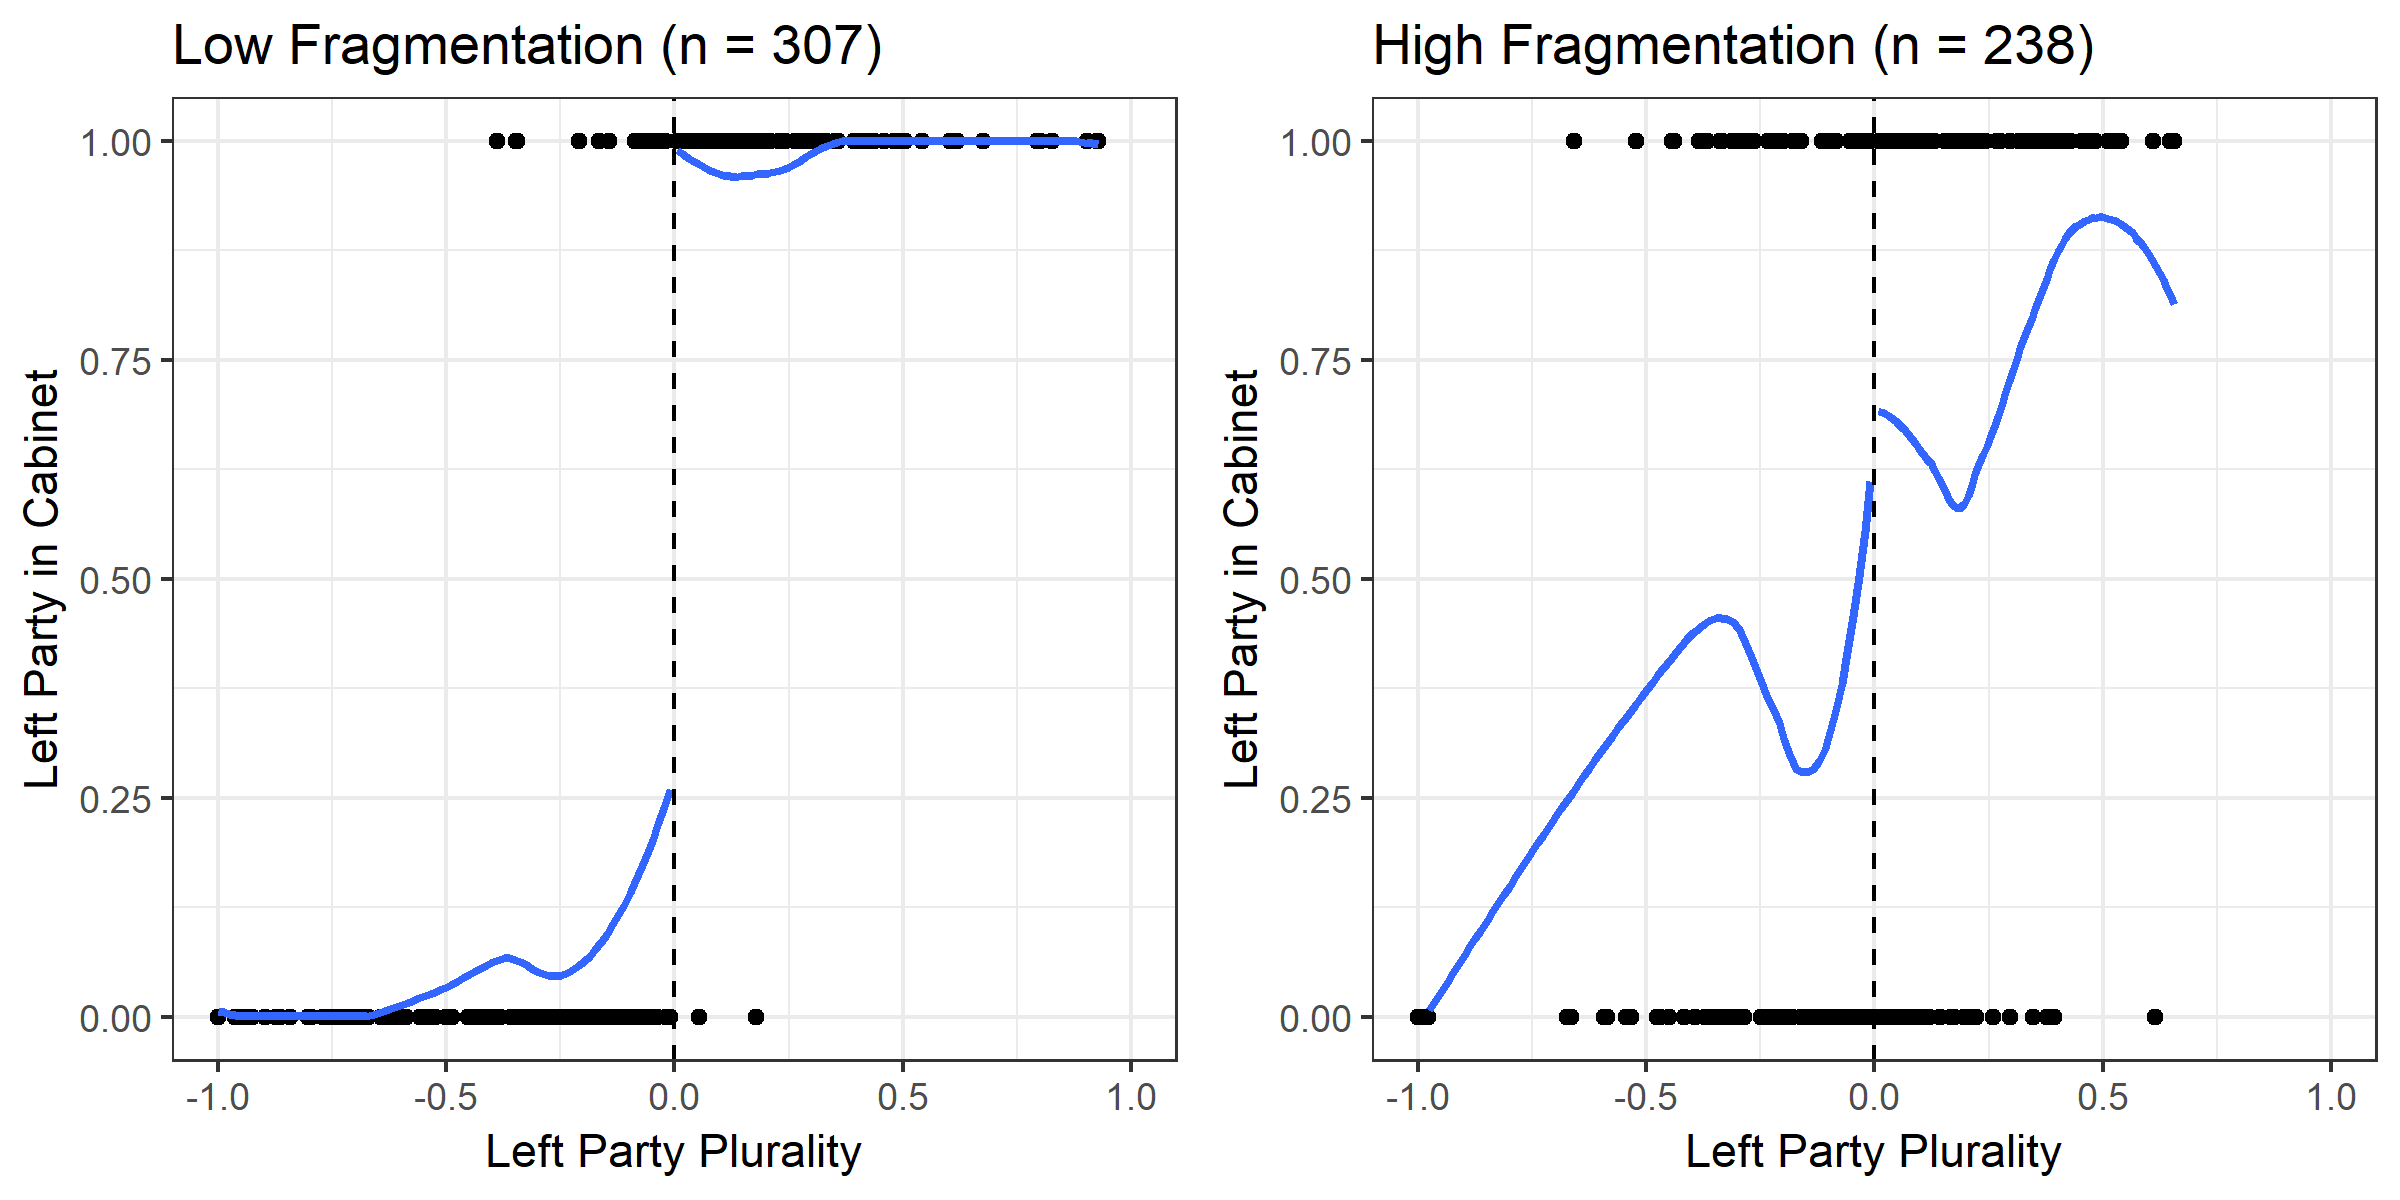
\includegraphics[width=\linewidth]{Figures/firstStageFigure}
\caption{When party fragmentation is low ($ENPP < 3.5$), there is a sharp discontinuity in the probability of left parties entering government when they achieve a plurality of seats in parliament. When party fragmentation is high ($ENPP > 3.5$), there is no such discontinuity.}
\label{fig:firststagefigure}
\end{figure}

% Table created by stargazer v.5.2.2 by Marek Hlavac, Harvard University. E-mail: hlavac at fas.harvard.edu
% Date and time: Fri, Nov 16, 2018 - 2:02:49 PM
\begin{table}[h] \centering 
  \caption{First-stage regression discontinuity estimates (bias-corrected) with 95\% confidence intervals (robust standard errors) in brackets.} 
  \label{table:firstStageRD} 
\begin{tabular}{@{\extracolsep{5pt}}lccc} 
\\[-1.8ex]\hline 
\hline \\[-1.8ex] 
 & \multicolumn{3}{c}{\textit{Fragmentation:}} \\ 
\cline{2-4} 
\\[-1.8ex] & All & Low & High \\ 
\\[-1.8ex] & (1) & (2) & (3)\\ 
\hline \\[-1.8ex] 
 Local Average Treatment Effect & 0.233 & 0.575 & 0.037 \\ 
  & [-0.035, 0.50] & [0.35, 0.80] & [-0.35, 0.42] \\ 
\hline \\[-1.8ex] 
Observations & 551 & 309 & 242 \\ 
Bandwidth Estimate $(h)$ & 0.175 & 0.218 & 0.181 \\ 
\hline 
\hline \\[-1.8ex] 
\end{tabular} 
\end{table} 


\subsection{Balance Tests}

%TODO Hartman and Hidalgo (2016) Balance Test Procedure?
The RD design relies on a crucial identifying assumption: the treatment must be the only variable that changes discontinuously at the threshold. If there are any other covariates that do so, then one cannot attribute a discontinuity in the outcome to the treatment alone. We perform a number of tests to ensure that pre-treatment covariates meet this continuity condition. For each covariate, we estimate a local-linear RD (triangular kernel), testing whether the difference in expected value at the threshold is significantly different than zero. The covariates we test include GDP per capita, Polity score, population, central government debt per capita, government expenditures, tax revenue per capita, annual inflation, and OECD average bond yields. The latter test is to ensure that our main results are not being driven by global movements in the bond market, but by country-specific bond price changes. 

As Figure \ref{fig:balanceplots} illustrates, there are no significant discontinuities for any of these covariates, with the exception of government expenditures -- elections with slight SD pluralities tend to be in countries with slightly \textit{lower} central government expenditures as a percentage of GDP. Although this seems unlikely to be the cause of a discontinuity in bond yield \textit{changes}, as a robustness check we will include a variant of the RD estimator that conditions on covariates, as proposed by \citet{Calonico2018} in Appendix \ref{appendix:robustness}. This test yields results that are similar to those in the primary analysis.

\begin{figure}
\centering
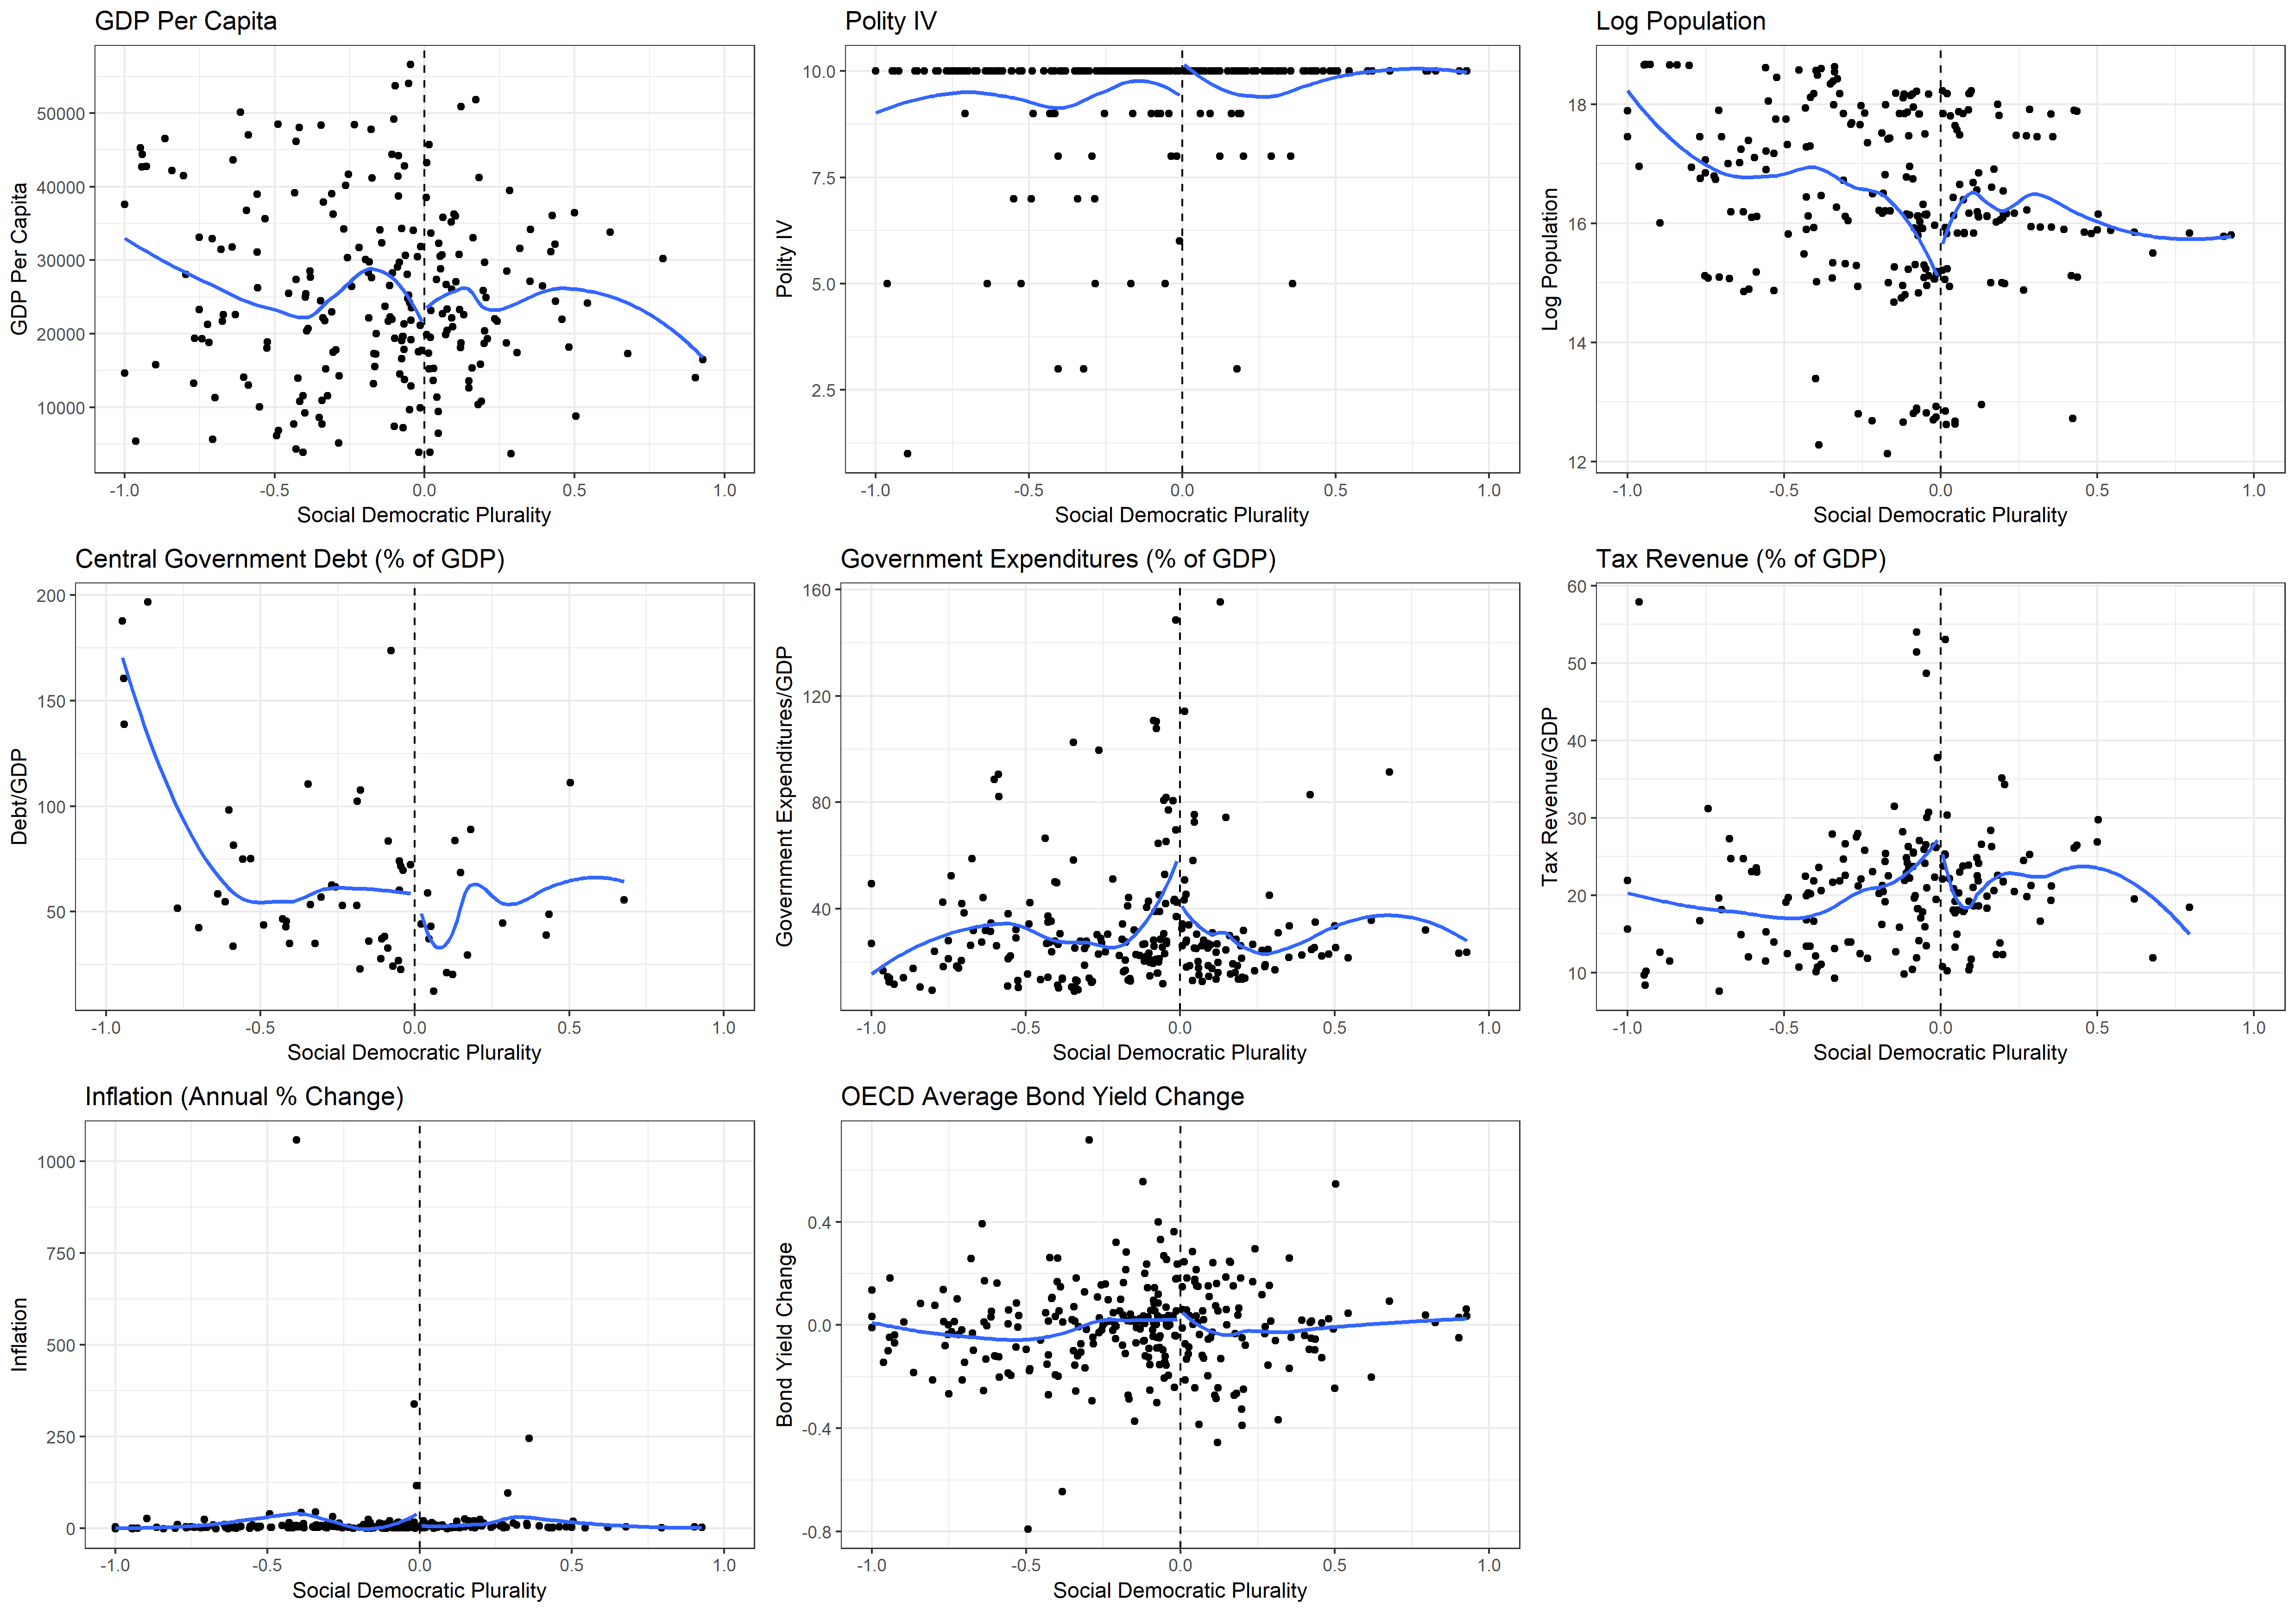
\includegraphics[width=\linewidth]{Figures/balancePlots}
\caption{For nearly every pre-treatment covariate, there is no significant discontinuity at the threshold. Note that these tests are conducted for elections with low party fragmentation, as in the primary analysis, but the finding holds when looking at the entire sample as well.}
\label{fig:balanceplots}
\end{figure}


\subsection{Bond Markets}

For the following analysis, we compute bias-corrected local-linear RD estimates with robust confidence intervals \citep{Calonico2014}. Table \ref{table:InterestRateRD} reports the estimated Local Average Treatment Effect (LATE), varying party fragmentation. In countries with High Fragmentation, there is no statistically significant discontinuity in bond yields at the threshold. But in countries with Low Fragmentation, there is a roughly half a percentage point increase in bond yields one month after the narrow election of a Left party. This is a striking result, and precisely what our mechanism predicts.

\begin{figure}[h]
\centering
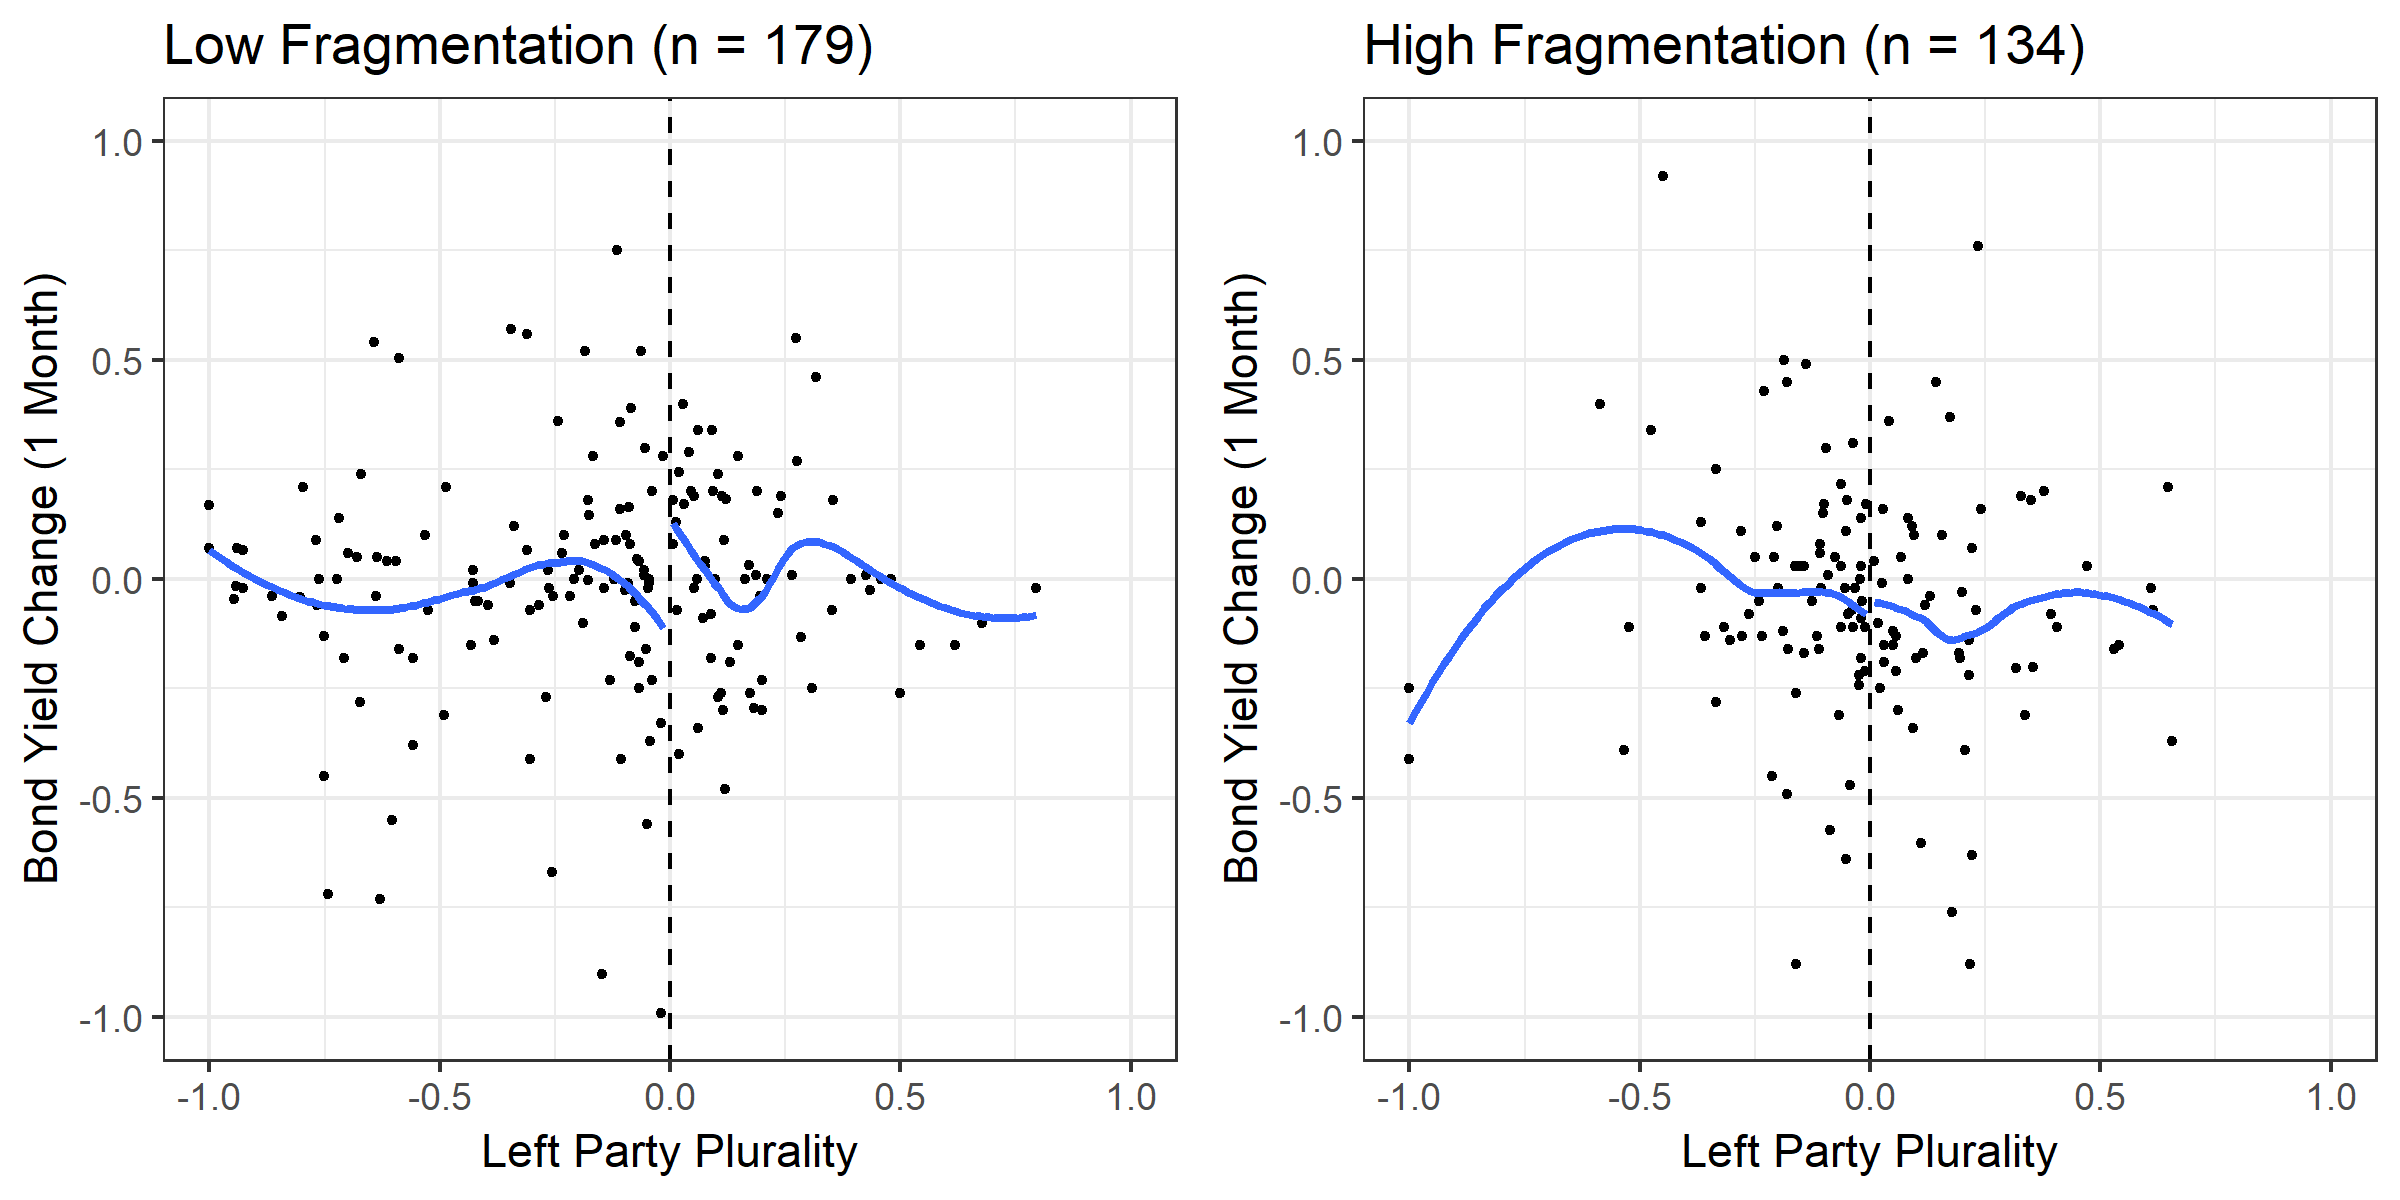
\includegraphics[width=\linewidth]{Figures/interestRateRDFigure}
\caption{Interest rate change 1 month after election, plotted against the plurality margin of the largest social democratic party.}
\label{fig:interestraterdfigure}
\end{figure}

% Table created by stargazer v.5.2.2 by Marek Hlavac, Harvard University. E-mail: hlavac at fas.harvard.edu
% Date and time: Fri, Nov 16, 2018 - 2:02:49 PM
\begin{table}[h] \centering 
  \caption{1-month bond yield regression discontinuity estimates (bias-corrected) with 95\% confidence intervals (robust standard errors) in brackets.} 
  \label{table:InterestRateRD} 
\begin{tabular}{@{\extracolsep{5pt}}lccc} 
\\[-1.8ex]\hline 
\hline \\[-1.8ex] 
 & \multicolumn{3}{c}{\textit{Fragmentation:}} \\ 
\cline{2-4} 
\\[-1.8ex] & All & Low & High \\ 
\\[-1.8ex] & (1) & (2) & (3)\\ 
\hline \\[-1.8ex] 
 Local Average Treatment Effect & 0.145 & 0.592 & $-0.048$ \\ 
  & [-0.12, 0.41] & [-0.01, 1.19] & [-0.32, 0.23] \\ 
\hline \\[-1.8ex] 
Observations & 316 & 179 & 137 \\ 
Bandwidth Estimate $(h)$ & 0.137 & 0.141 & 0.125 \\ 
\hline 
\hline \\[-1.8ex] 
\end{tabular} 
\end{table}  


\subsection{Dynamic RD Estimates} %TODO Sticky Note: Does this make sense?

In addition to estimating the short-run effects on bond yields, we can compute a \textit{dynamic} RD estimate by varying the time window with which the dependent variable is measured \citep{Cellini2010}. Using this method, we can observe whether a social democratic plurality yields long-term changes to bond yields. And as a placebo test, we also observe whether there an estimated effect on bond yields \textit{prior} to the election. Figure \ref{fig:dynamicRD} illustrates the results from the dynamic RD analysis; the narrow election of a left party appears to have an effect on bond yields that persist for at least a year when party fragmentation is low, and not when it is high. 

\begin{figure} [h]
	\centering
	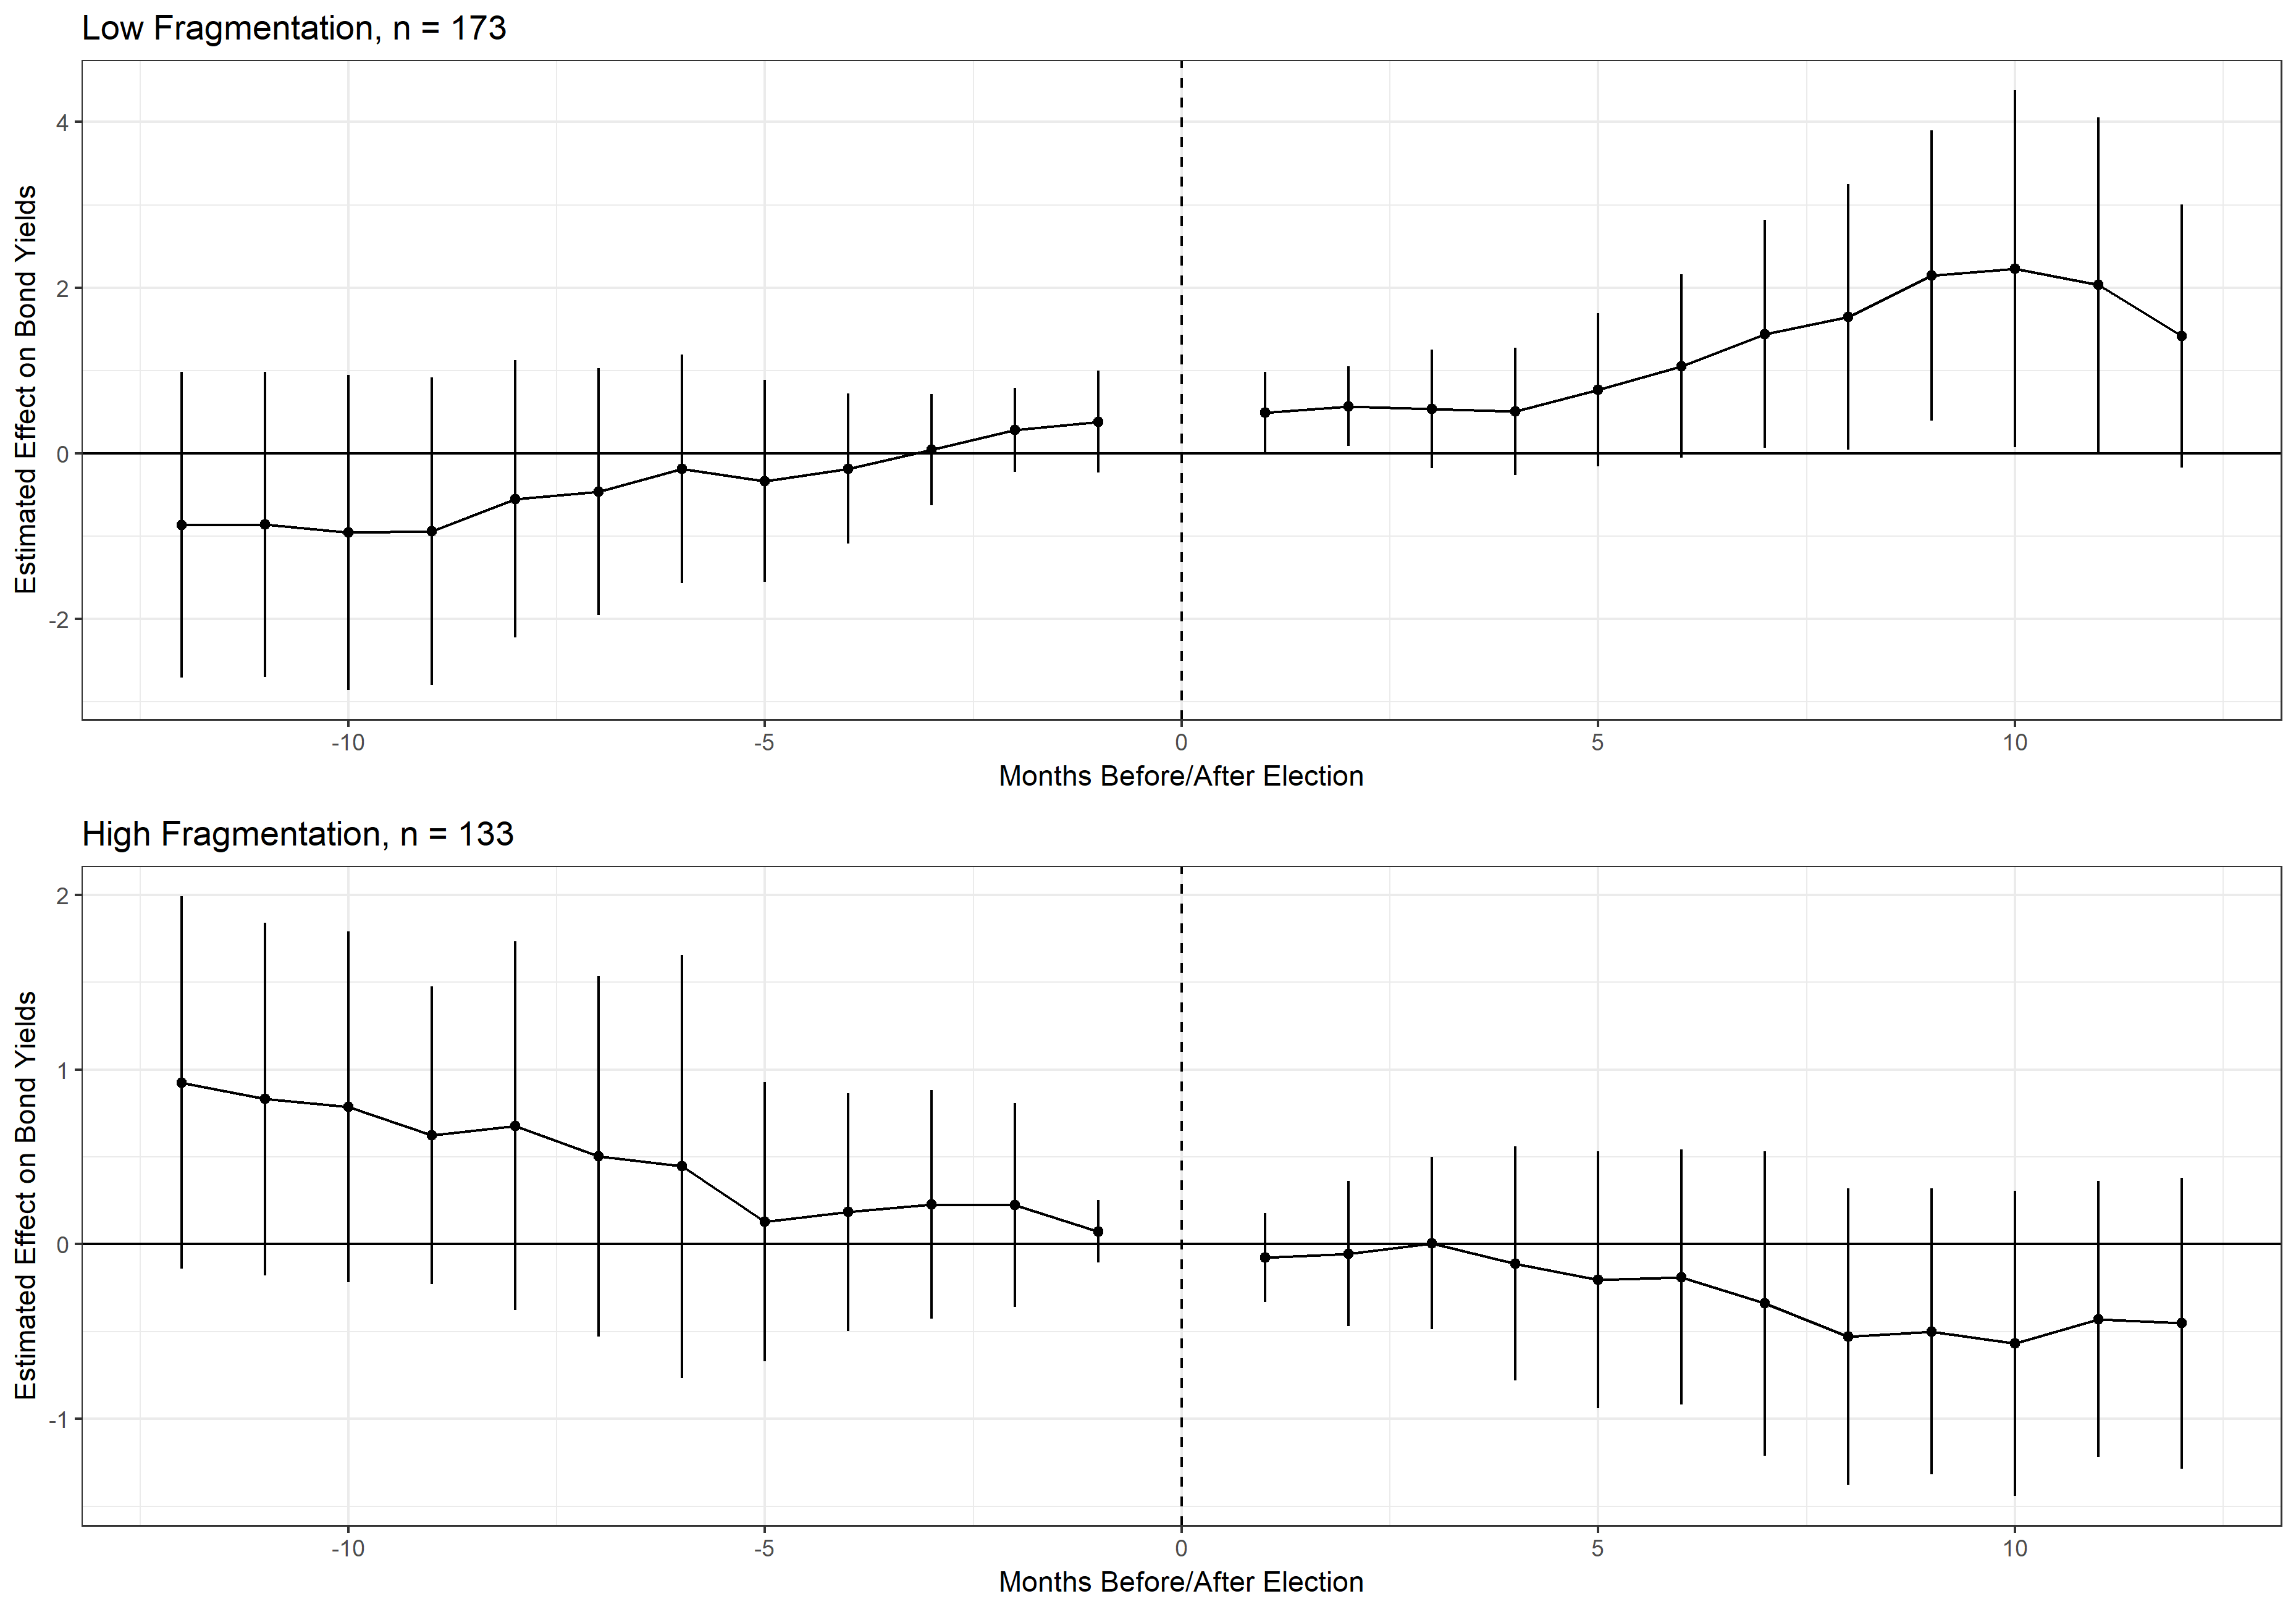
\includegraphics[width=\linewidth]{Figures/dynamicRD}
	\caption{Dynamic RD estimates. Top panel is low fragmentation elections ($ENPP < 3.5$), bottom panel is high fragmentation elections ($ENPP > 3.5$).}
	\label{fig:dynamicRD}
\end{figure}

\section{Heterogeneous Treatment Effects}

The strength of the bond market response to social democratic government is likely to depend on the counterfactual. What is the identity of the government that \textit{would} have formed if social democrats had not won a plurality? We would expect bond market movements to be strongest when the party that lost the plurality was, for instance, strongly conservative. Whereas, if both parties vying for the plurality were left parties, then financial markets would have already anticipated a left government, and would have priced government bonds accordingly. To explore this hypothesis, we test how the RD estimate varies with the absolute difference between the two parties' ideal points on ParlGov's ideology score. Figure \ref{fig:rdEstimateVaryingIdeologyDistance} plots this change. There is some evidence that the treatment effect is larger when we restrict ourselves to looking at cases where the absolute difference in ideology score is large (e.g., greater than 3). But a word of caution: the sample sizes on those estimates start to get pretty small ($n = 69$).

\begin{figure}[h]
	\centering
	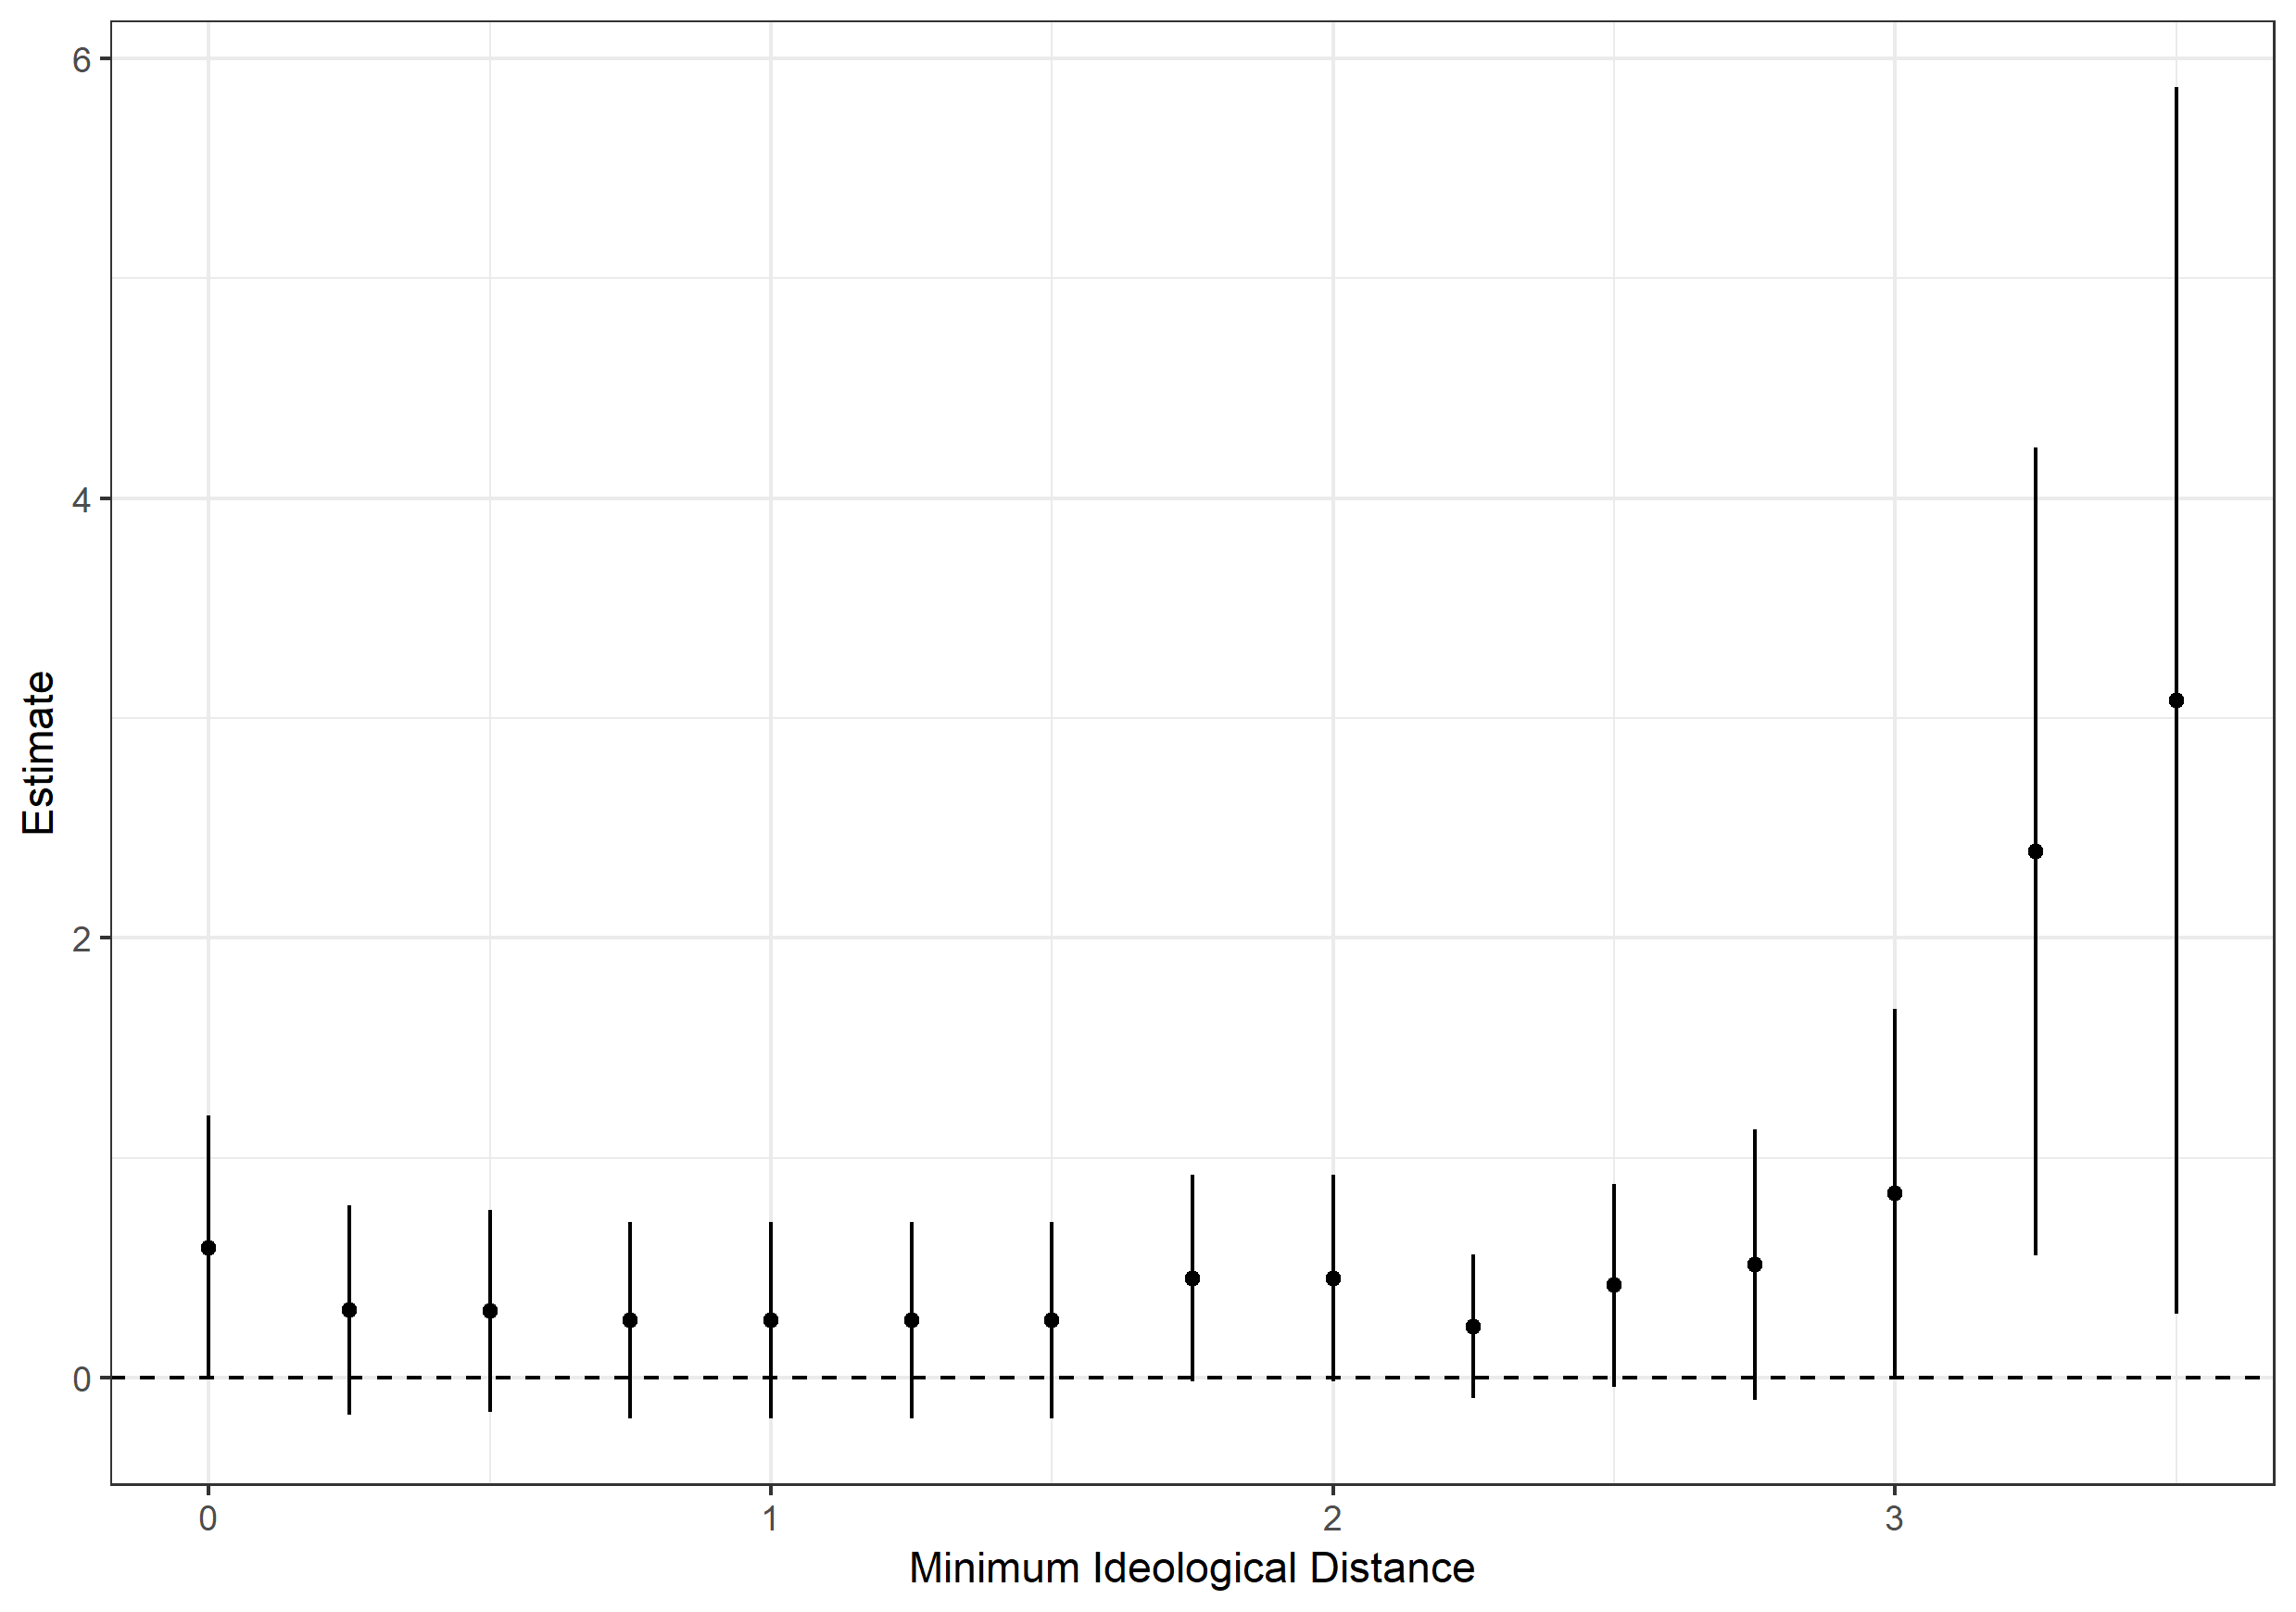
\includegraphics[width=\linewidth]{Figures/rdEstimateVaryingIdeologyDistance}
	\caption{As we restrict our estimation to elections where the two largest parties were far apart from one another in ideological distance, the estimated treatment effect grows.}
	\label{fig:rdEstimateVaryingIdeologyDistance}
\end{figure}

Figure \ref{fig:rdEstimateVaryingYear} illustrates how the estimated effect varies over time -- each point reports an estimate and confidence interval from a 30-year window. In the period of fixed exchange rates and low capital mobility (pre-1976), the effect of social democracy on interest rates is large. But post-1976, the effect appears to shrink, consistent with Rodrik's ``golden straightjacket'' hypothesis. 

%TODO Sticky Note: This is what we expected, right??
\begin{figure}
\centering
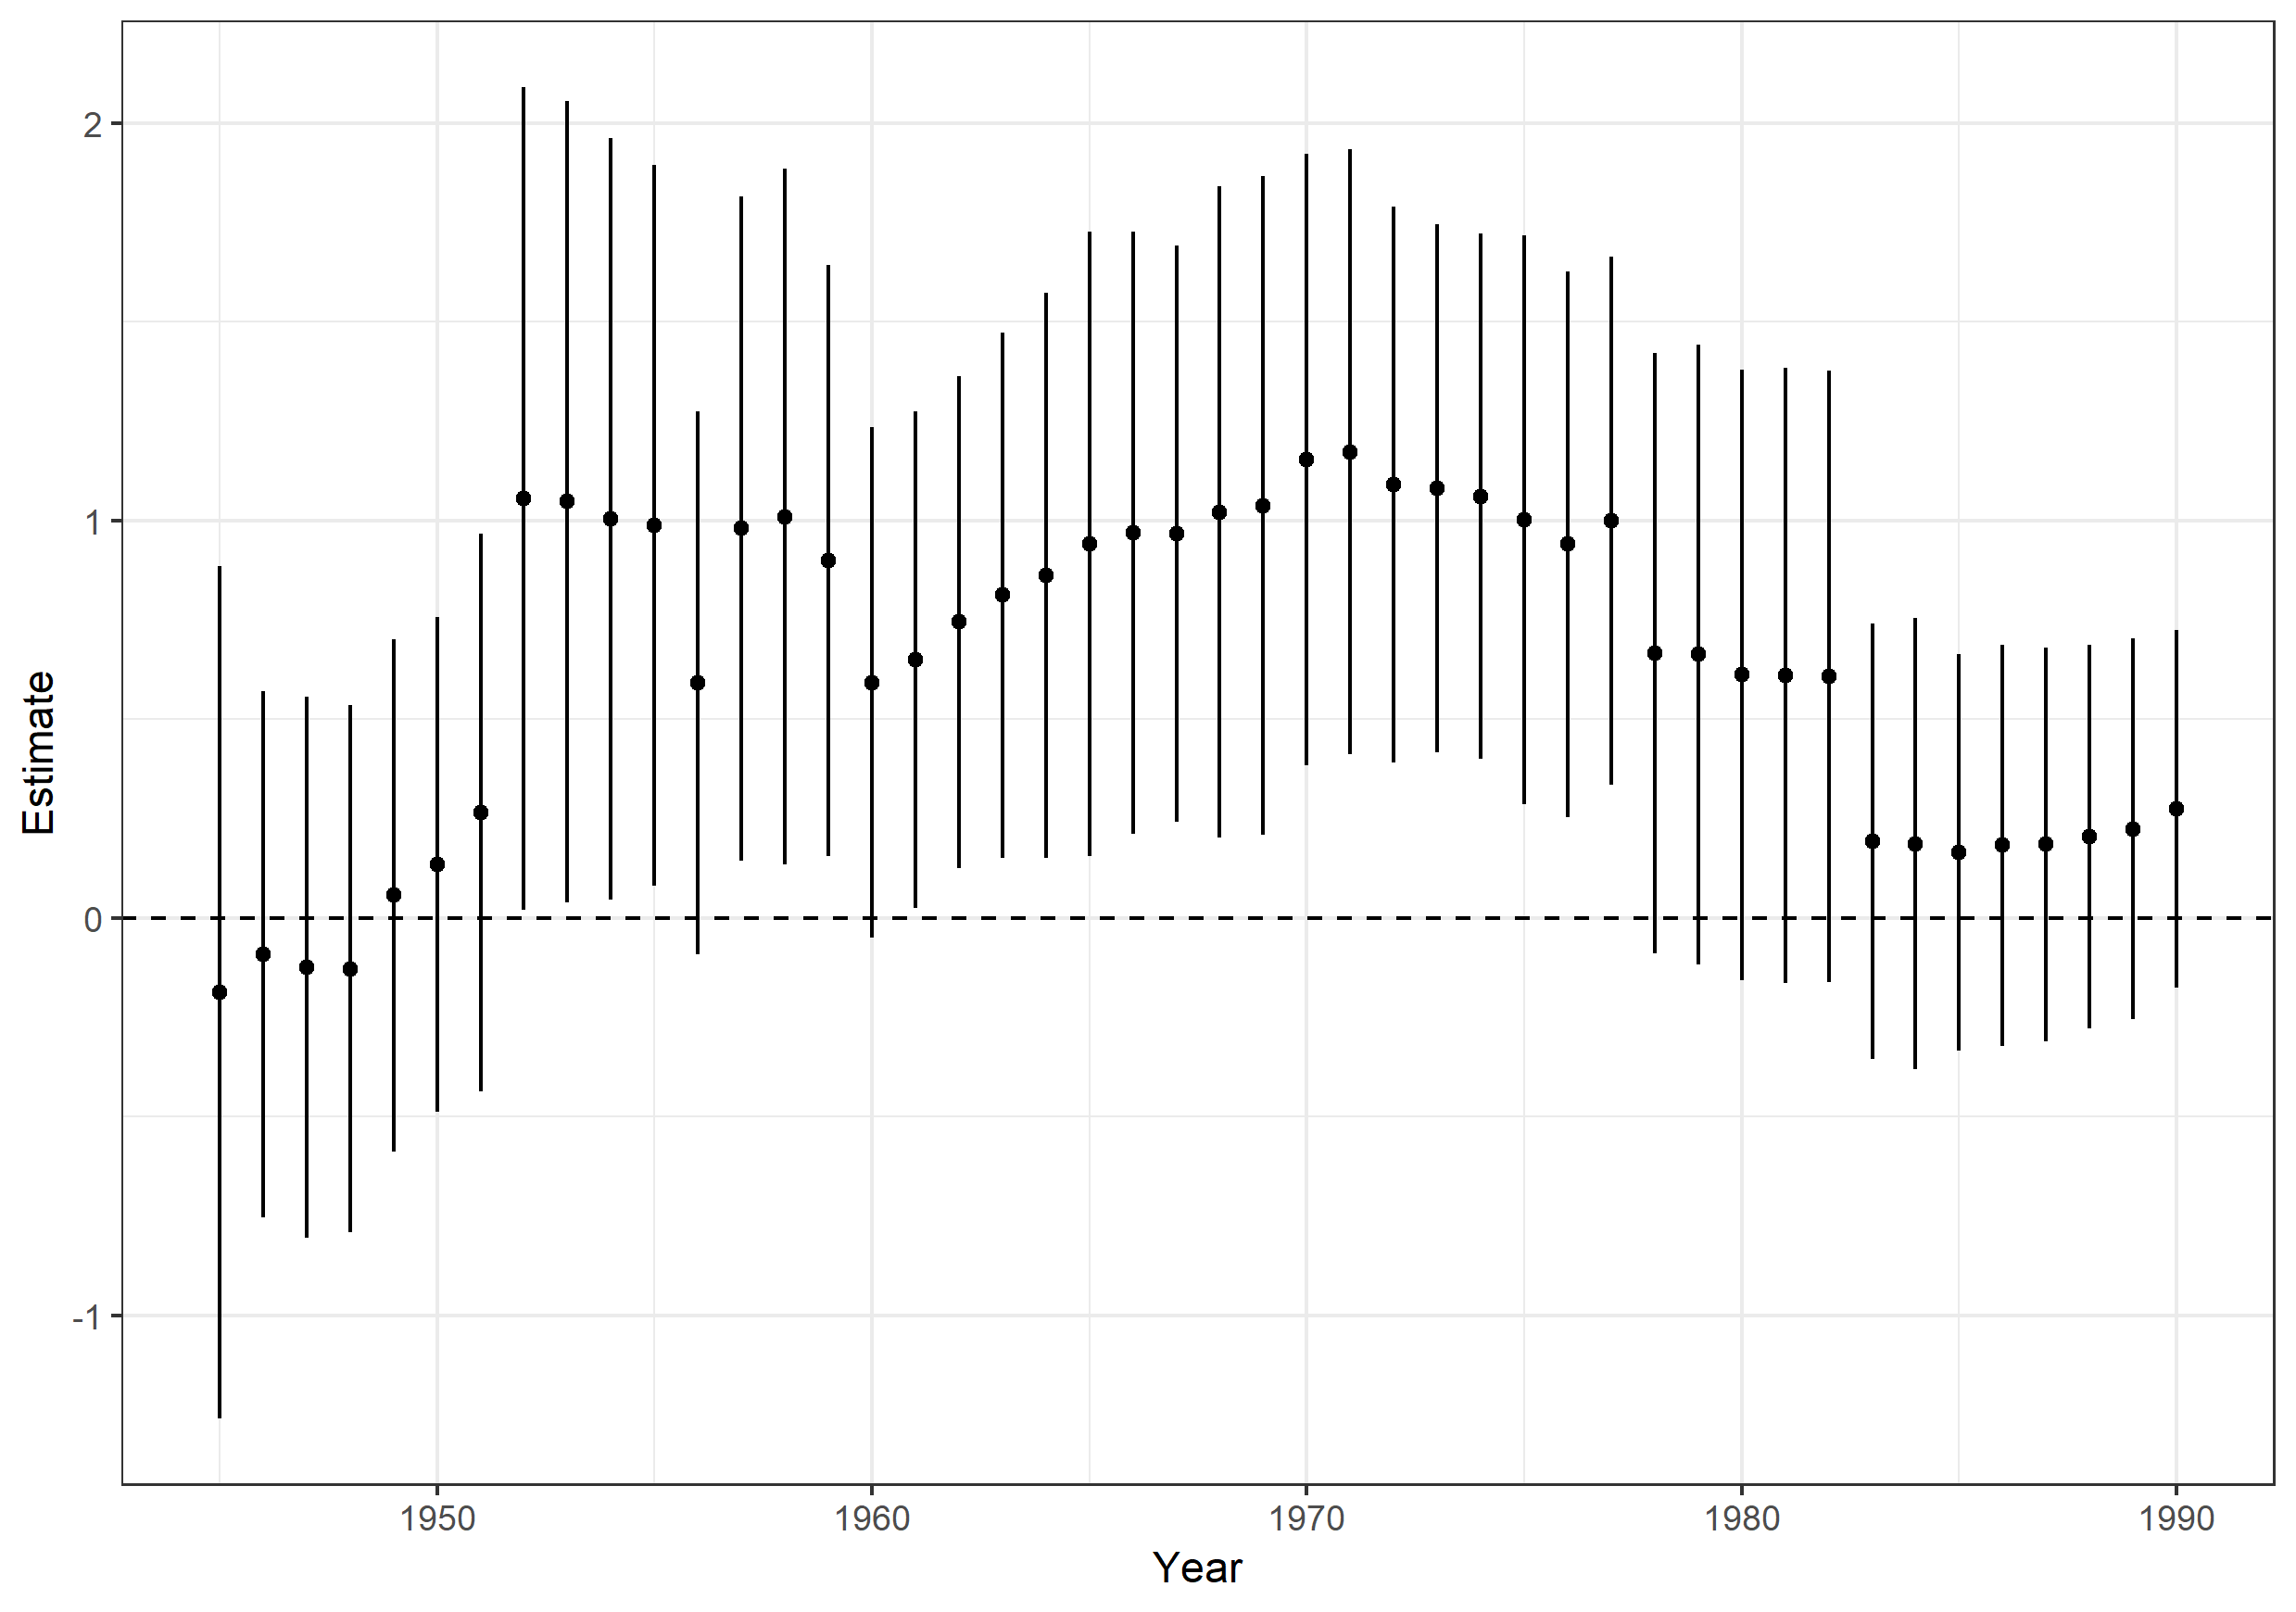
\includegraphics[width=\linewidth]{Figures/rdEstimateVaryingYear}
\caption{The RD estimate seems to shrink in later years (Each point is estimated using 30 years of data; x-axis denotes the minimum year.)}
\label{fig:rdEstimateVaryingYear}
\end{figure}

%TODO Sticky Note on Political Institutions


\section{Conclusion}
%TODO Sticky Note on Conclusion


\bibliography{refs}


\begin{appendices}
	
	
	\section{Robustness Tests} \label{appendix:robustness}
	
	\subsection{Varying the ENPP Threshold}
	Figure \ref{fig:rdEstimateVaryingENPP} illustrates how the RD estimate and 95\% confidence interval changes when we vary the ENPP threshold. The result is fairly robust to our choice of threshold, though when it is less than 3 the effective sample size is much smaller, and the robust standard errors much larger. 
	
	\begin{figure}[h]
		\centering
		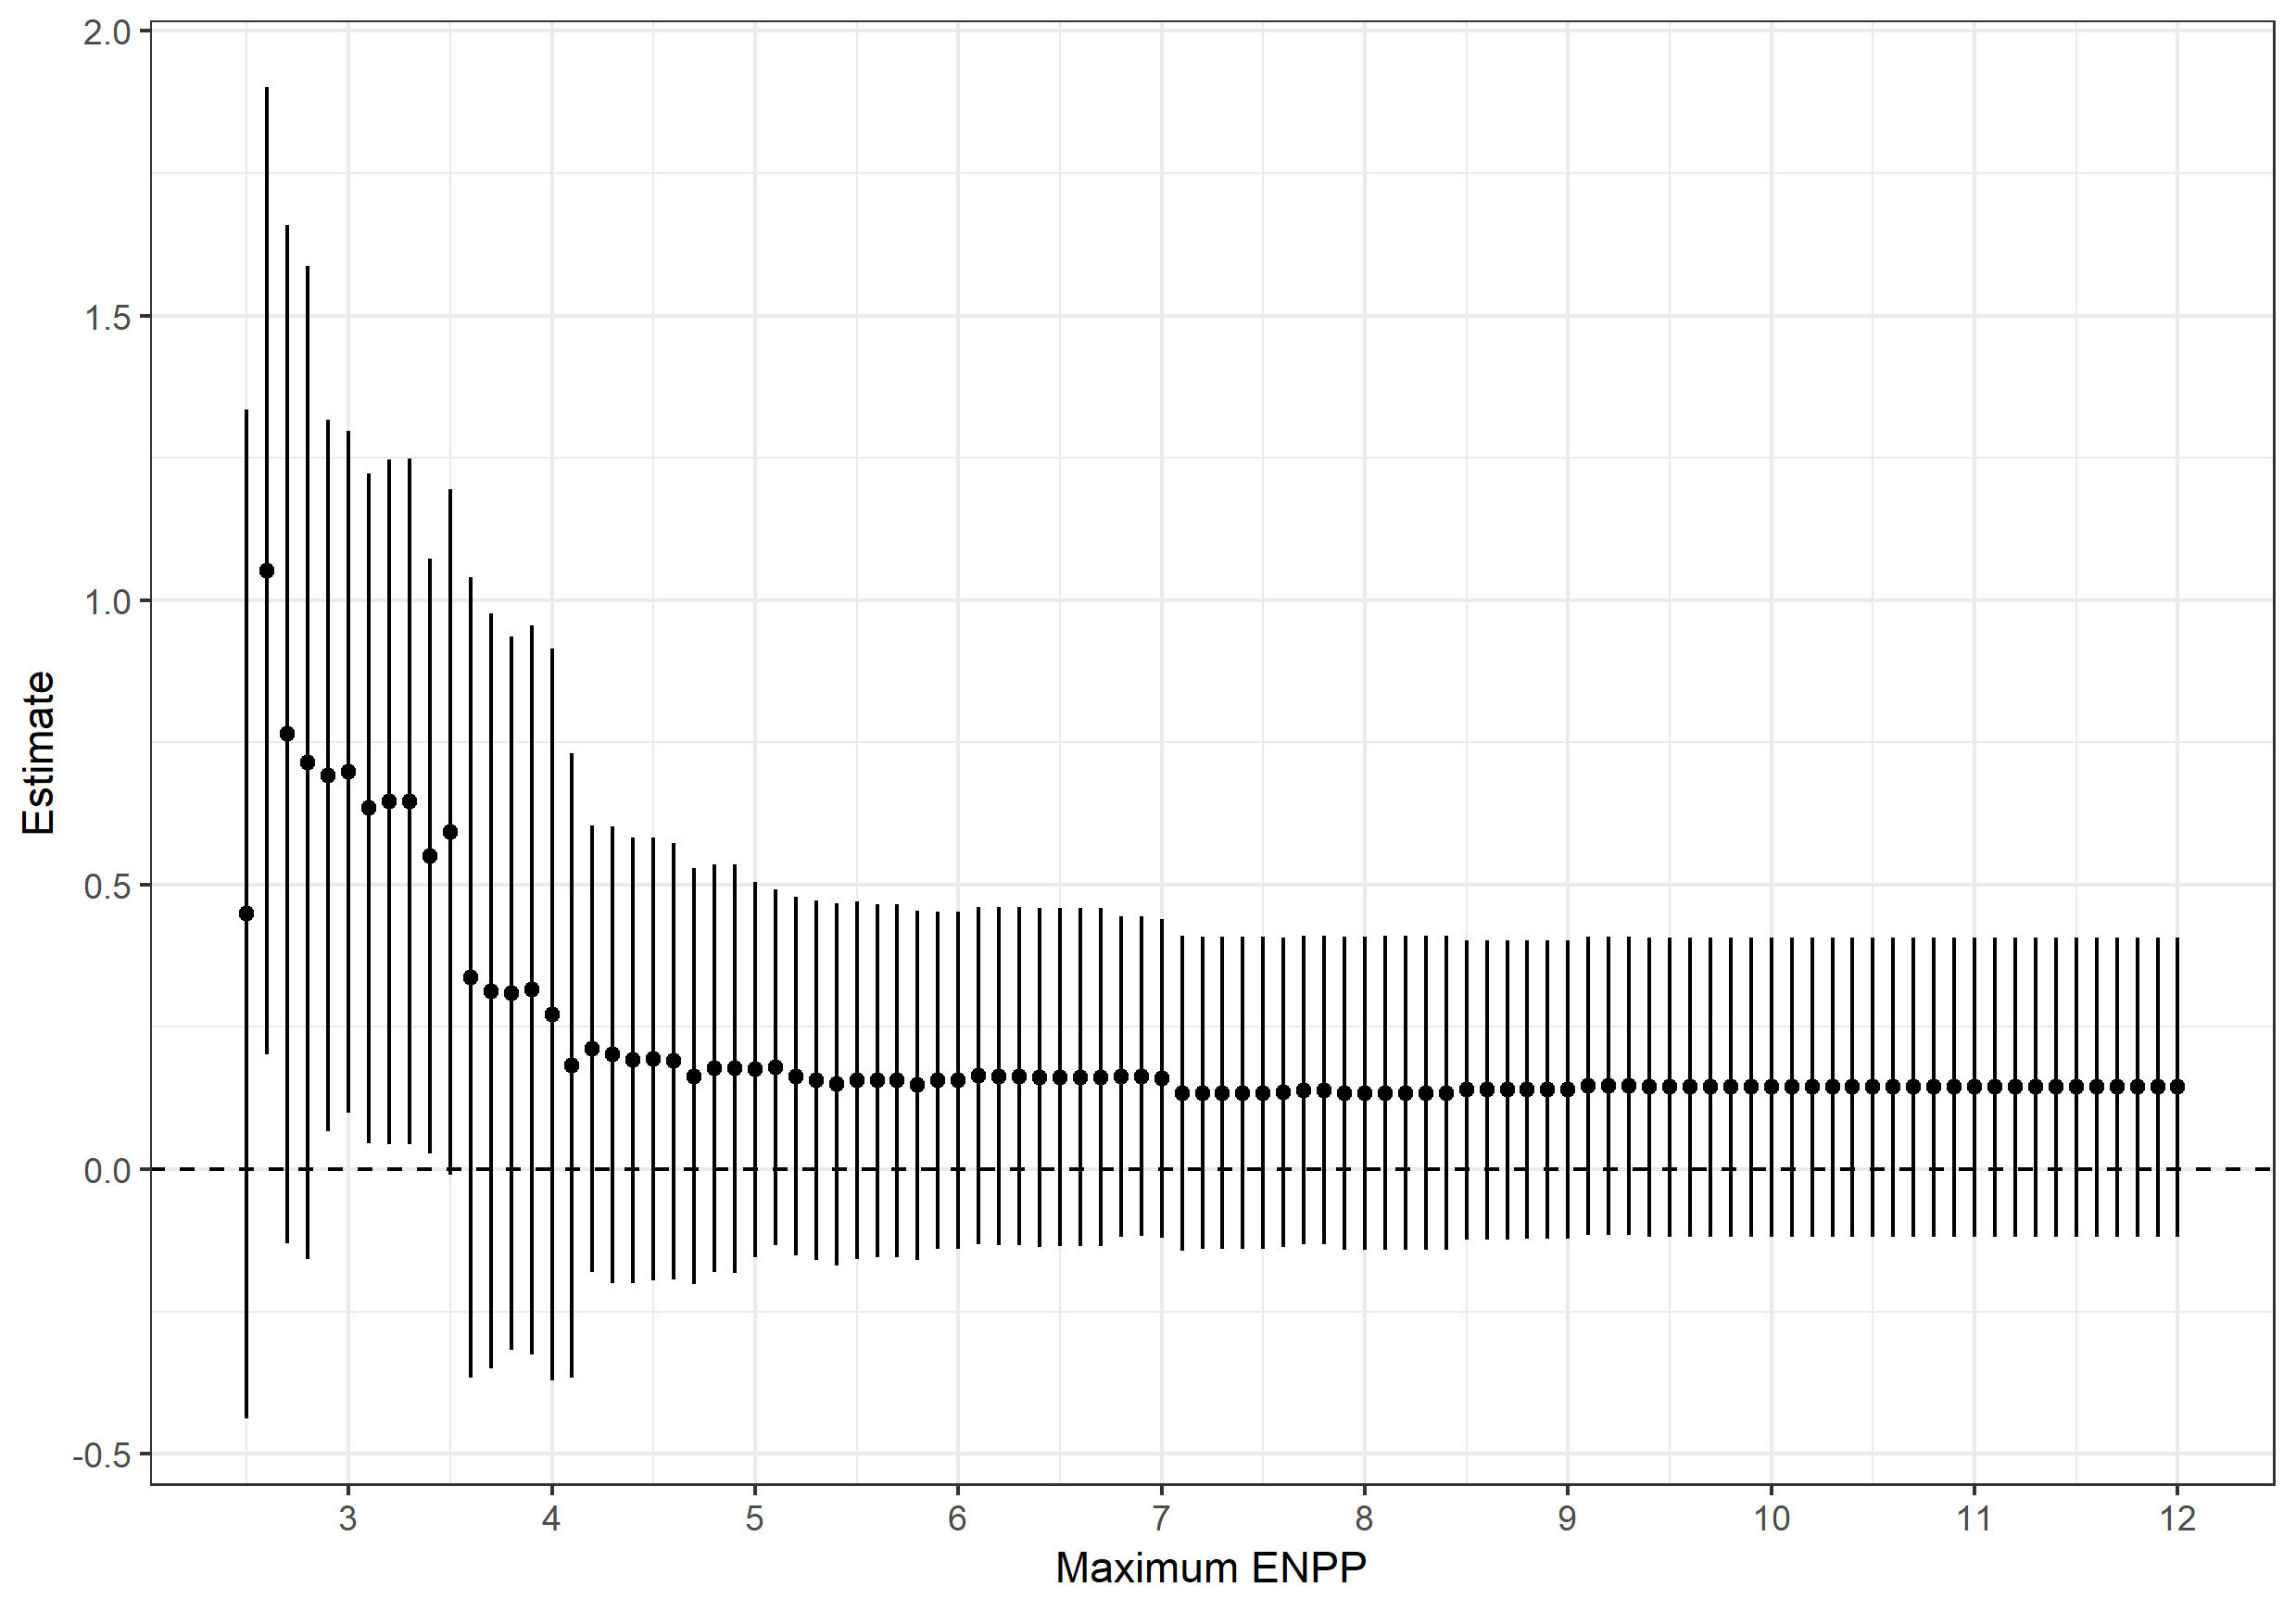
\includegraphics[width=\linewidth]{Figures/rdEstimateVaryingENPP}
		\caption{Estimated treatment effects and 95\% confidence intervals, varying the ENPP threshold. The estimate is largest when party fragmentation is low (ENPP $< 3.5$)}
		\label{fig:rdEstimateVaryingENPP}
	\end{figure}

	\subsection{Regression Discontinuity with Covariates}
	
	\citet{Calonico2018} propose a procedure to adjust for covariates in a regression discontinuity framework. Estimating using this procedure -- conditioning on GDP per capita, log population, expenditures per capita, tax revenue as a percentage of GDP, and inflation -- yields the results in Table \ref{table:RDWithCovariates}. 
	
	% Table created by stargazer v.5.2.2 by Marek Hlavac, Harvard University. E-mail: hlavac at fas.harvard.edu
	% Date and time: Fri, Nov 16, 2018 - 2:02:49 PM
	\begin{table}[h] \centering 
		\caption{Regression discontinuity with pre-treatment covariates. Dependent variable = 1-month bond yield regression discontinuity estimates (bias-corrected) with 95\% confidence intervals (robust standard errors) in brackets.} 
		\label{table:RDWithCovariates} 
		\begin{tabular}{@{\extracolsep{5pt}}lccc} 
			\\[-1.8ex]\hline 
			\hline \\[-1.8ex] 
			& \multicolumn{3}{c}{\textit{Fragmentation:}} \\ 
			\cline{2-4} 
			\\[-1.8ex] & All & Low & High \\ 
			\\[-1.8ex] & (1) & (2) & (3)\\ 
			\hline \\[-1.8ex] 
			Local Average Treatment Effect & 0.146 & 1.01 & $-0.146$ \\ 
			& [-0.14, 0.43] & [0.46, 1.56] & [-0.45, 0.16] \\ 
			\hline \\[-1.8ex] 
			Observations & 236 & 118 & 118 \\ 
			Bandwidth Estimate $(h)$ & 0.138 & 0.135 & 0.129 \\ 
			\hline 
			\hline \\[-1.8ex] 
		\end{tabular} 
	\end{table}  


	\subsection{Sensitivity to Bandwidth}
	
	As Figure \ref{fig:bandwidthSensitivity} illustrates, our result is somewhat sensitive to choice of bandwidth. Using a smaller bandwidth than the CCT optimum yields significantly fewer observations near the cutoff, increasing standard errors. And the local-linear estimate shrinks with larger bandwidths (as would be expected, judging from the chart in Figure \ref{fig:interestraterdfigure}.) 
	
	
	\begin{figure}[h]
	\centering
	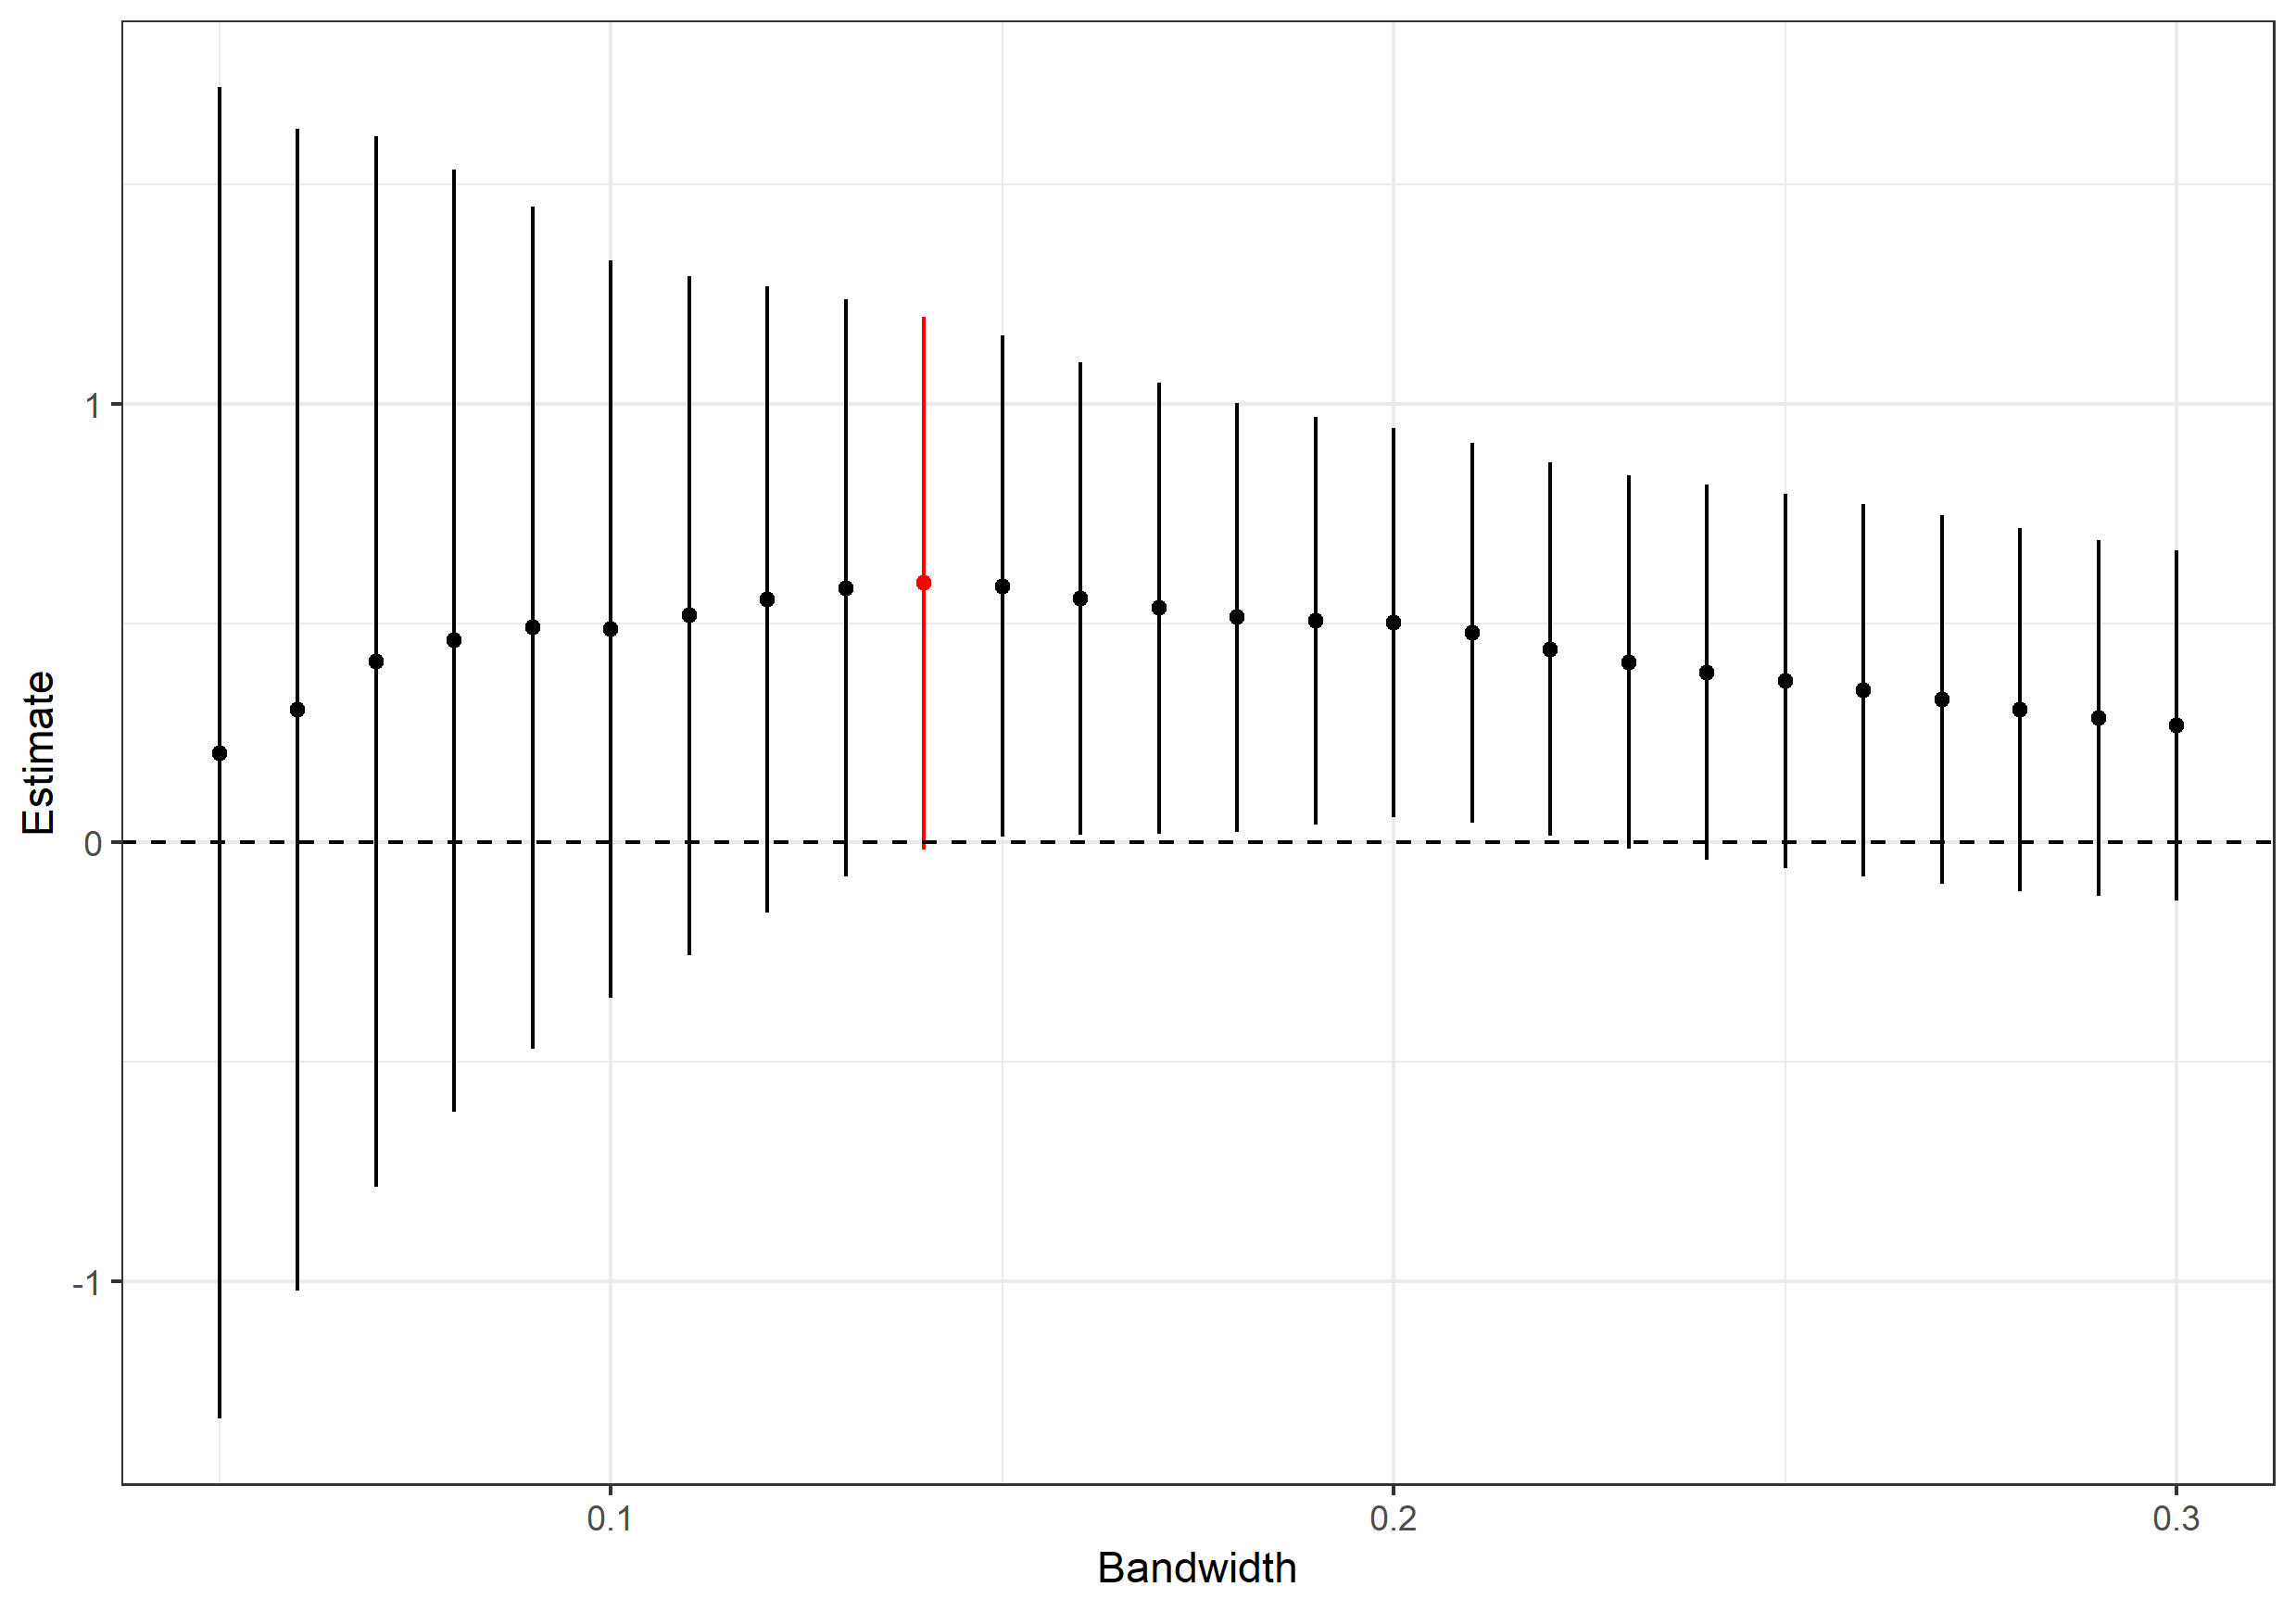
\includegraphics[width=\linewidth]{Figures/bandwidthSensitivity}
	\caption{Sensitivity to choice of bandwidth. Bias-corrected estimates and 95\% confidence intervals (robust standard errors). The CCT optimal bandwidth is plotted in red.}
	\label{fig:bandwidthSensitivity}
	\end{figure}

	\subsection{Sensitivity to Polynomial Order and Kernel Function}

	The \texttt{rdrobust} package defaults to modeling the conditional expectation function with a local-linear and triangular kernel weights. The core result is robust to varying these assumptions, though the 95\% confidence interval is wider (and includes zero) when estimated using a second-order polynomial.
	 
	% Table created by stargazer v.5.2.2 by Marek Hlavac, Harvard University. E-mail: hlavac at fas.harvard.edu
	% Date and time: Fri, Nov 16, 2018 - 2:02:49 PM
	\begin{table}[h] \centering 
		\caption{Regression discontinuity estimates, varying polynomial order and kernel function. Dependent variable = 1-month bond yield regression discontinuity estimates (bias-corrected) with 95\% confidence intervals (robust standard errors) in brackets.} 
		\label{table:RDQuadratic} 
		\begin{tabular}{@{\extracolsep{5pt}}lccc} 
			\\[-1.8ex]\hline 
			\hline \\[-1.8ex] 
			& \multicolumn{3}{c}{\textit{Fragmentation:}} \\ 
			\cline{2-4} 
			\\[-1.8ex] & All & Low & High \\ 
			\\[-1.8ex] & (1) & (2) & (3)\\ 
			\hline \\[-1.8ex] 	
			Linear, Triangular Kernel & 0.145 & 0.592 & $-0.048$ \\ 
			& [-0.12, 0.43] & [-0.01, 1.19] & [-0.32, 0.23] \\ 
			Linear, Uniform Kernel & 0.152 & 0.511 & $-0.077$ \\ 
			& [-0.20, 0.39] & [0.10, 0.92] & [-0.39, 0.23] \\ 
			Quadratic, Triangular Kernel & 0.099 & 0.646 & $-0.109$ \\ 
			& [-0.20, 0.39] & [$-0.11$, 1.40] & [-0.43, 0.21] \\ 
			Quadratic, Uniform Kernel & 0.106 & 0.598 & 0.016 \\ 
			& [-0.19, 0.41] & [$-0.14$, 1.33] & [-0.31, 0.34] \\ 
			\hline \\[-1.8ex] 
			Observations & 316 & 179 & 137 \\ 
			%Bandwidth Estimate $(h)$ & 0.203 & 0.241 & 0.152 \\ 
			\hline 
			\hline \\[-1.8ex] 
		\end{tabular} 
	\end{table}  

\end{appendices}





\end{document}